% !TEX TS-program = lualatex
% !TEX encoding = UTF-8 Unicode
% --- Preamble: Styling ---
\documentclass[a4paper,12pt]{article}
\usepackage[left=3cm,top=3cm,bottom=2cm,right=2cm]{geometry}

% Encoding & Language
\usepackage[utf8]{inputenc}
\usepackage[T1]{fontenc}
\usepackage[portuguese]{babel}
\addto\extrasportuguese{\renewcommand{\contentsname}{Índice}}

% Margins, Columns, Indentation & Spacing
\usepackage{multicol}
\usepackage{indentfirst}
\usepackage{ragged2e}  % For extendability
\usepackage{setspace}
\onehalfspacing
\setlength{\columnsep}{1cm}

% Headers, Titles, Footnotes & Captioning
\usepackage{sectsty}
\usepackage{titling}
\renewcommand\maketitlehooka{\null\mbox{}\vfill}
\renewcommand\maketitlehookd{\vfill\null}
\usepackage{footmisc}
\usepackage{caption}
\captionsetup[figure]{font=footnotesize}

% Graphics Support
\usepackage{graphicx}
\graphicspath{{./assets/}}
\usepackage{svg}
\usepackage{tikz}
\usepackage{float}
\usepackage{fancyhdr}
\usepackage{xcolor}
\usetikzlibrary{shapes,shadows,arrows,positioning,calc}
\tikzstyle{RectObject}=[rectangle,fill=white,draw,line width=0.5mm]
\tikzstyle{line}=[draw]
\tikzstyle{arrow}=[draw, -latex]

% --- Preamble: Commands ---
\pagestyle{fancy}
\fancyhf{}
\fancyfoot[R]{\thepage}
\renewcommand{\headrulewidth}{0pt}

% --- Document: Begin ---
\begin{document}
% --- Document: Title Page ---
\begin{titlingpage}
    \begin{center}
        {\large
            % Institution
            {\Huge
                FATEC -- Prof. Waldomiro May
            }\\
            ANÁLISE E DESENVOLVIMENTO DE SISTEMAS

            % Project Presentation
            \vspace{1cm}
            SEMANA DE TECNOLOGIA

            % Project Logo
            \vspace{6cm}
            \raisebox{-0.75em}{
\includegraphics[scale=0.1]{neotasker-logo.png}}
            % Project Name
            {\Huge
                \textbf{NeoTasker}
            }

            % Project Description
            Agenda Pessoal

            % Authors
            \vspace{2cm}
            CHRYSTIAN M. FRANKLIN \\
            WELLINGTON E. RODRIGUES

            % Date
            \vspace{8cm}
            2023.2
        }
    \end{center}
\end{titlingpage}

% --- Document: Table of Contents ---
\setcounter{tocdepth}{4}
\tableofcontents
\pagebreak

% --- Document: Table of Figures ---
\listoffigures
\pagebreak

% --- Document: Content ---
% --- Segment: Introduction ---
\section{Introdução}
\subsection{Tema}
O software \textbf{NeoTasker} é um \textit{Sistema de Gerenciamento de Agenda Pessoal}. Este caracteriza-se pelo controle de atividades e eventos decorrentes do dia-a-dia de um indivíduo.

\subsection{Justificativa de Escolha do Tema}
A organização pessoal é uma tarefa árdua e frequentemente mais complexa do que imaginada, especialmente quando é considerado as rotinas frenéticas de estudantes e trabalhadores, devido ao seu vasto e variado uso de tempo, com suas rotinas crescentemente mais corridas.

A partir dessa consideração, o tema de \textbf{agenda pessoal} foi selecionado devido à familiaridade do ambiente dos autores, em conjunto com as possibilidades de diferentes soluções relacionadas ao aspecto de controle de tempo e organização de rotinas.

\subsection{Descrição do Problema}
O sistema deve ser capaz de efetuar o agendamento, modificação, consultas e remoção dos diferentes tipos de atividades presentes de maneira individual. Além de apresentar relatórios e informações estatísticas sobre as atividades e o uso do sistema, visando melhorar a experiência do usuário em relação a sua organização de tempo.

\subsection{Objetivos do Projeto}
Este projeto é caracterizado por ser uma atividade conjunta com o objetivo de desenvolver os conteúdos das seguintes disciplinas do segundo período do curso de análise e desenvolvimento de sistemas:
\begin{itemize}
    \item \textbf{IES100:} Engenharia de Software I;
    \item \textbf{IHC001:} Interação Humano Computador;
    \item \textbf{ILP010:} Linguagem de Programação;
    \item \textbf{ISI002:} Sistemas de Informação.
\end{itemize}

Além do aspecto disciplinar, este projeto tem como objetivos secundários o desenvolvimento de habilidades essenciais no atual ambiente de trabalho:
\begin{itemize}
    \item A produção de um projeto relacionado ao \textbf{Gerenciamento de Tempo e Rotina};
    \item A execução da \textbf{Metodologia Ágil} e \textbf{SCRUM};
    \item A \textbf{Análise de Projetos} e o \textbf{Levantamento de Requisitos};
    \item A \textbf{Consideração de Aspectos de Acessibilidade};
    \item A \textbf{Produção de Documentação e Manuais};
    \item O \textbf{Desenvolvimento de Sistemas de Softwares Completos};
    \item A \textbf{Implementação de Caso de Testes}.
\end{itemize}

\subsection{Organização do Projeto}
\subsubsection{Estrutura do Projeto}
O projeto está estruturado a partir da organização de projetos em cascatas, com base na seguinte visão:

\vspace{1em}
\begin{figure}[H]
    \centering
    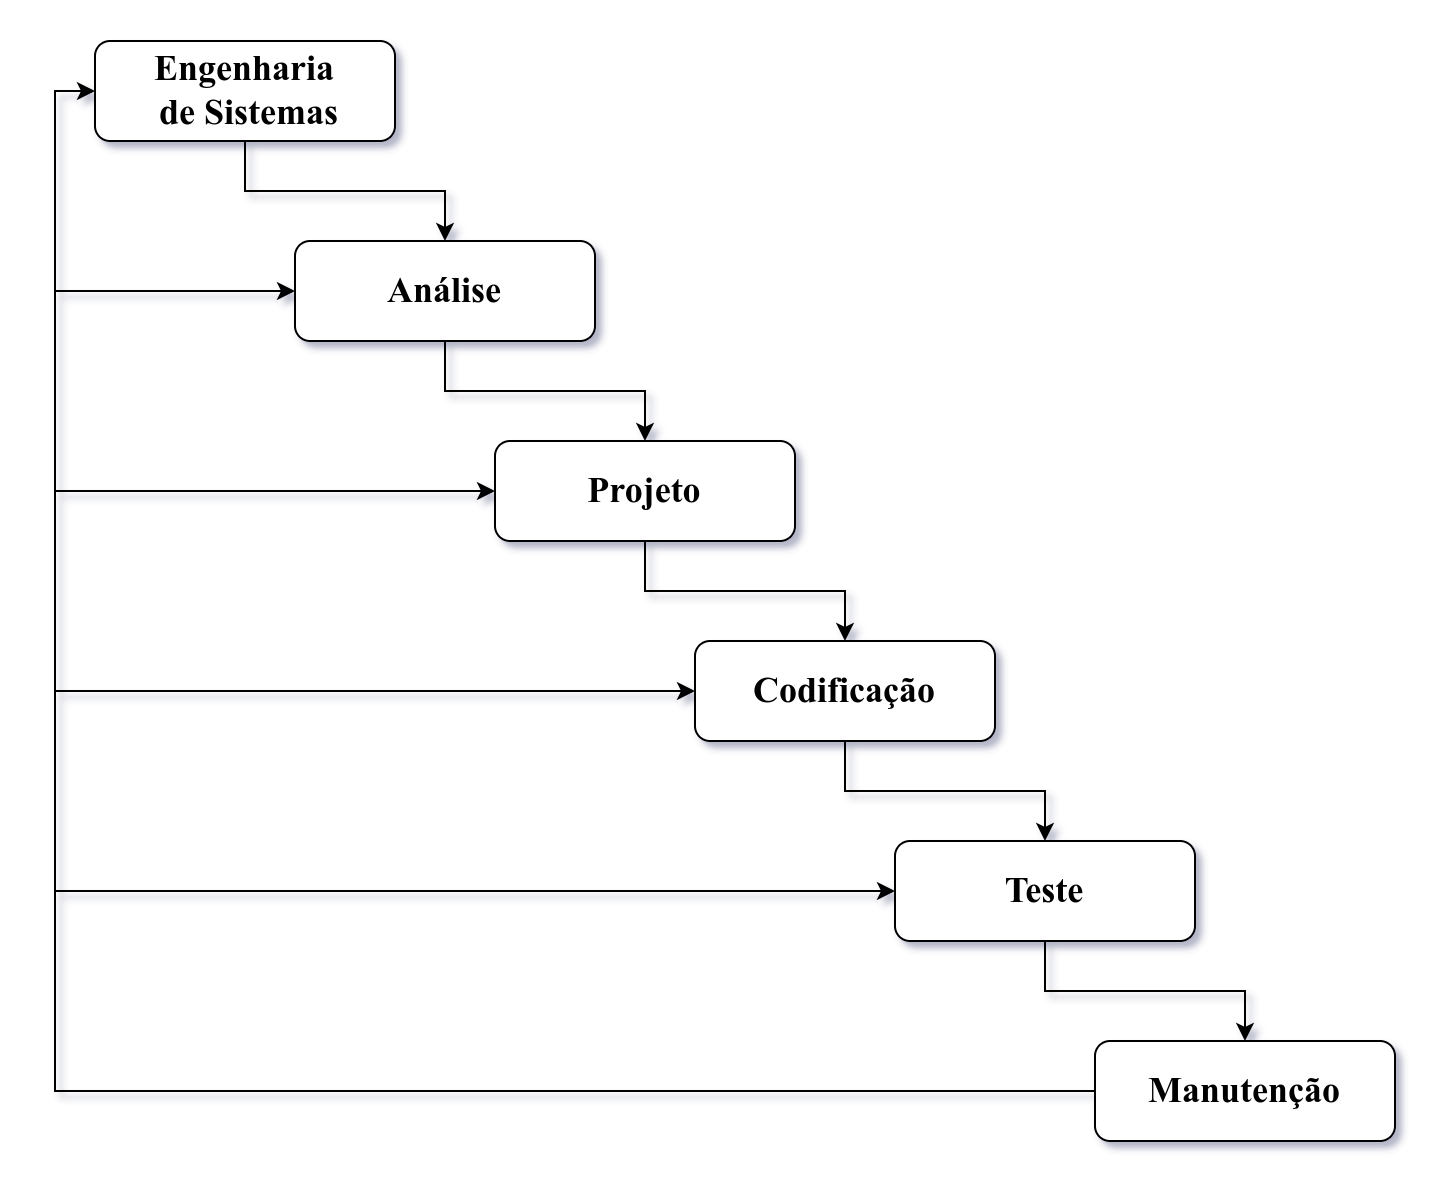
\includegraphics[scale=0.25]{waterfall.drawio.png}
    \caption{Desenvolvimento em Cascata}
\end{figure}

Esta estrutura é o que permite que o desenvolvimento ocorra de maneira crescente e parcial, onde cada adição, extensão, modificação ou remoção de componentes resulte na adaptação da documentação e código, voltando ao ponto de desenvolvimento no qual a mudança ocorreu, garantindo assim uma maior estabilidade e qualidade de produto.

\subsubsection{Método de Trabalho}
O Método Ágil com SCRUM\footnote{
    Criado por \textbf{Jeff Sutherland} em 1990.
} foi empregado para orientar os desenvolvimentos dos diferentes processos presentes na estrutura do projeto. Utilizado também no mercado de trabalho, o método incorpora as atividades de levantamento de requisitos, análise, projetos \textit{(prototipação)}, implementação/evolução, e entrega.

As atividades individuais são organizadas em \textbf{Sprints}, que delimitam um certo período de tempo -- \textit{geralmente de uma a duas semanas} -- desde o início até o fim do processo.

\subsubsection{Divisão de Responsabilidades}
O projeto consta com dois membros, portanto, as atividades estão substituídas da seguinte maneira:

\paragraph{Chrystian M. Franklin}
\begin{itemize}
    \item Planejamento e Estruturação do Projeto;
    \item Construção de Documentação e Manuais;
    \item Controle do Versionamento;
    \item Correção de Bugs e Otimizações;
    \item Implementação de Casos de Testes Automatizados;
    \item Desenvolvimento dos Aspectos Back-End.
\end{itemize}

\paragraph{Wellington E. Rodrigues}
\begin{itemize}
    \item Design e Padrões de Cores;
    \item Organização e Distribuição de Atividades e Responsabilidades;
    \item Levantamento de Requisitos e Features Adicionais;
    \item Consideração de Itens de Acessibilidade;
    \item Construção de Diagramas e Protótipos Gráficos;
    \item Desenvolvimento dos Aspectos Front-End.
\end{itemize}

% --- Segment: Requirements ---
\section{Levantamento de Requisitos}
\textbf{Levantamente de Requisitos} é a prática onde se estuda e debate as funcionalidades que deverão ser contempladas no sistema, além das regras para tais funcionalidades e os cenários de implantação. Todo esse estudo, compreende na \textbf{Engenharia de Sistemas} que oferece suporte e abrange todas as atividades relacionadas à investigação, definição e delimitação de novos sistemas ou modificações. Essa etapa é crucial no processo de desenvolvimento de software, no qual o engenheiro de requisitos, o analista de negócios, e o engenheiro de sistemas ou desenvolvedor de software trabalham juntos para identificar as necessidades e requisitos do cliente. Uma vez que os requisitos do sistema são identificados, os projetistas de sistemas estão prontos para criar a solução.

Na etapa de \textbf{Levantamento de Requisitos} temos a deinfição de três tipos de requisitos, onde cada um deles possuem suas características próprias. Os requisitos são:
\begin{itemize}
	\item Requisitos Funcionais;
	\item Requisitos Não-Funcionais; e
	\item Requisitos de Domínio.
\end{itemize}



\subsection{Requisitos Funcionais}
Os \textbf{Requisitos Funcionais} são aqueles que indicam quais as funcionalidades o sistema possuirá, ou seja, o que o sistema é capaz de executar e processar com as informações. Exemplos são:
\begin{itemize}
	\item Capacidade de cadastramento de usuários;
	\item Capacidade de geração de relatório mensal de vendas; e
	\item Capacidade de exportar os dados em arquivos.
\end{itemize}

\subsection{Requisitos Não-Funcionais}
Os \textbf{Requisitos Não-Funcionais} são aqueles que quais as obrigações ou regras que devem ser aplicadas para que as funcionalidades descritas nos Requisitos Funcionais estejam em conformidade com a necessidade do cliente.
Outra aplicação dos \textbf{Requisitos Não-Funcionais} é quanto a limitação do sistema, ou seja, o que ele não deve fazer em hipótese alguma. Exemplos são:
\begin{itemize}
	\item Tempo execução de ações do sistema menor do que 2 segundos; e
	\item Compatibilidade do sistema com sistemas operacionais (caso uma aplicação desktop) ou com versões de navegadores (caso uma aplicação web).
\end{itemize}


\subsection{Requisitos de Domínio}
Os \textbf{Requisitos de Domínio} são aqueles que buscam alinhar o domínio do cliente, ou seja, o ambiente/segmeto de mercado que está inserido e ao qual o \textit{software} desenvolvido será inserido. Exemplos são:
\begin{itemize}
	\item A geração de relatórios deve ser feita sempre filtrando pelo dados mais recentes e com maiores índices; e
	\item O sistema somente ficará disponível para emissões de notas em horário comercial.
\end{itemize}

% --- Segment: Data Flow Diagrams ---
\section{Diagrama de Fluxo de Dados}
Os \textbf{Diagramas de Fluxo de Dados} são os diagramas que representam como os dados percorrem por entre os processos e por quais processos. Cada Requisito Funcional deve apresentar um DFD (Diagrama de Fluxo de Dados) correspondente ao processo.

\section{Requisitos e DFDs}
\subsection{Requisitos Funcionais do Sistema}
\begin{figure}[H]
	\centering
	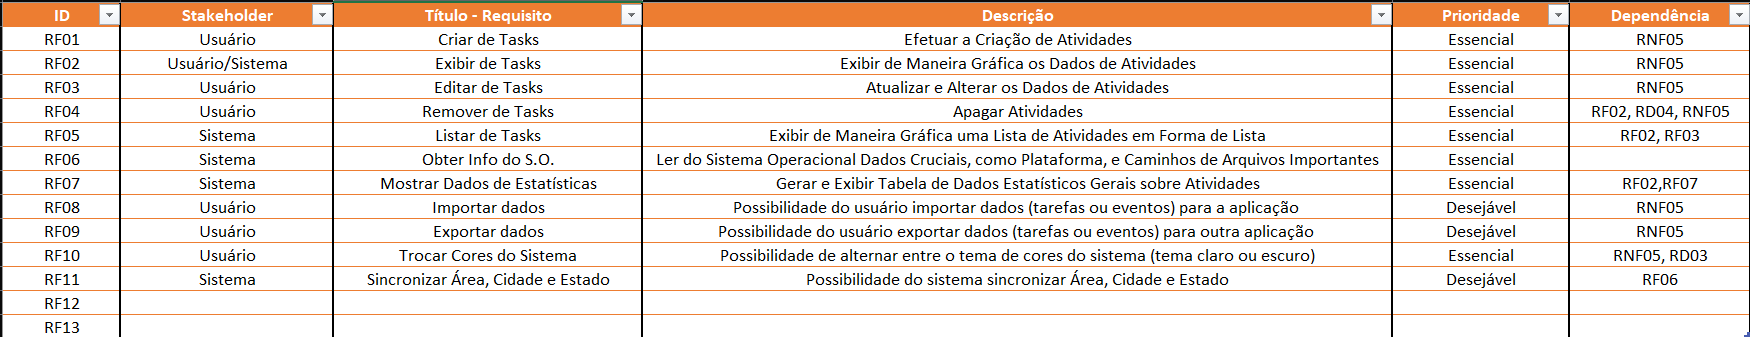
\includegraphics[scale=0.25]{requirements/requirements.png}
	\caption{DFD do RF00}
\end{figure}

\subsection{RF01 - Criar Tasks}
O sistema deve permitir que o usuário crie uma nova \textbf{Task}, onde o usuário deve informar o título da \textbf{Task}, a data de término da \textbf{Task}, sendo estes dois primeiros os dados obrigatórios para sua criação. Como dados opcionais, temos a data de início da \textbf{Task}, descrição da \textbf{Task}, repetição entre períodos e as tags da \textbf{Task}.
\begin{figure}[H]
	\centering
	\includegraphics[scale=0.25]{dfd/RF01.png}
	\caption{DFD do RF01}
\end{figure}

\subsection{RF02 - Visualizar Tasks}
O sistema deve permitir que o usuário visualize todas as \textbf{Tasks} já existentes, onde o usuário deve informar o título da \textbf{Task} a ser visualizada.
\begin{figure}[H]
	\centering
	\includegraphics[scale=0.25]{dfd/RF02.png}
	\caption{DFD do RF04}
\end{figure}

\subsection{RF03 - Editar Tasks}
O sistema deve permitir que o usuário edite uma \textbf{Task} já existente, onde o usuário deve informar o título da \textbf{Task}, a data de término da \textbf{Task}, sendo estes dois primeiros os dados obrigatórios para sua criação. Como dados opcionais, temos a data de início da \textbf{Task}, descrição da \textbf{Task}, repetição entre períodos e as tags da \textbf{Task}.
\begin{figure}[H]
	\centering
	\includegraphics[scale=0.25]{dfd/RF02.png}
	\caption{DFD do RF02}
\end{figure}

\subsection{RF04 - Excluir Tasks}
O sistema deve permitir que o usuário exclua uma \textbf{Task} já existente, onde o usuário deve informar o título da \textbf{Task} a ser excluída.
\begin{figure}[H]
	\centering
	\includegraphics[scale=0.25]{dfd/RF03.png}
	\caption{DFD do RF03}
\end{figure}

\subsection{RF05 - Listar Tags}
O sistema deve listar todas as \textbf{Tags} já existentes, em ordem de mais recentes para mais antigas.
\begin{figure}[H]
	\centering
	\includegraphics[scale=0.25]{dfd/RF05.png}
	\caption{DFD do RF05}
\end{figure}

\subsection{RF06 - Obter Infor do Sistema Operacional}
O sistema deve obter informações do sistema operacional, com qual é por exemplo.
\begin{figure}[H]
	\centering
	\includegraphics[scale=0.25]{dfd/RF06.png}
	\caption{DFD do RF06}
\end{figure}

\subsection{RF07 - Mostra Dados de Estatísticas}
O sistema deve mostrar dados de estatísticas, sendo o número de task criadas, concluídas, programadas e atrasadas.
\begin{figure}[H]
	\centering
	\includegraphics[scale=0.25]{dfd/RF07.png}
	\caption{DFD do RF07}
\end{figure}


\section{Dicionário de Dados}
O \textbf{Dicionário de Dados} é o documento ao qual é representado os tipos de dados, quais são eles e como serão representados dentro do sistema.

% --- Segment: Design ---
\section{Design}
% --- Segment: Prototypes ---
\subsection{Protótipos}
Prototipar é o processo ao qual uma versão básica do sistema, a fim de vizualizar qual seria o funcionamento do sistema ou que ele de fato poderia oferecer ao usuário final quanto a sua usabilidade do sistema, quanto as ferramentas e funcionalidade alinhadas na etapa de \textbf{Engenharia de Sistemas}, além de apresentar, o mais fielmente possível, os aspectos do front-end do sistema ou \textit{desing} das telas e relacionados.

Quanto ao funcionamento pensado, nossos sistema apresentaria todas as telas por meio de JPanels\footnote{
	Ferramenta de Organização de Painéis disponível no uso do Java Swing
}, a não ser a tela principal, que seria aplicado o uso de JFrames\footnote{
	Ferramenta de Organização de Telas (Frames) disponível no uso do Java Swing
}. A troca entre telas seria aplicada dinamicamente, de modo que a cada ação do usuário - ao clicar em um botão por exemplo - a tela correspondente seria aplicada sobre a tela atual, substituindo. Tal uso forneceria uma melhor usabilidade para o usuário, sem precisar se preocupar com a organização das telas no momento de inicialzação a cada evento.

\subsection{Tela Principal}
A \textbf{Tela Principal} seria o JFrame ao qual sempre seria atualizado os JPanels para cada ação correspondente do usuário, logo, os únicos componentes ou o único grupo de elementos seria a barra superior de navegação e pesquisa, presente em todo momento e em qualquer ação do sistema.

\subsubsection{Tema Claro}
Telas com tema claro são aquelas que apresentam cores mais claras, como o branco, o cinza claro, o azul claro, entre outros. A ideia de um tema claro é a de que o usuário possa utilizar o sistema em ambientes com iluminação mais forte, como em ambientes externos, por exemplo.
\begin{itemize}
	\item Tela Principal
	\begin{figure}[H]
		\centering
		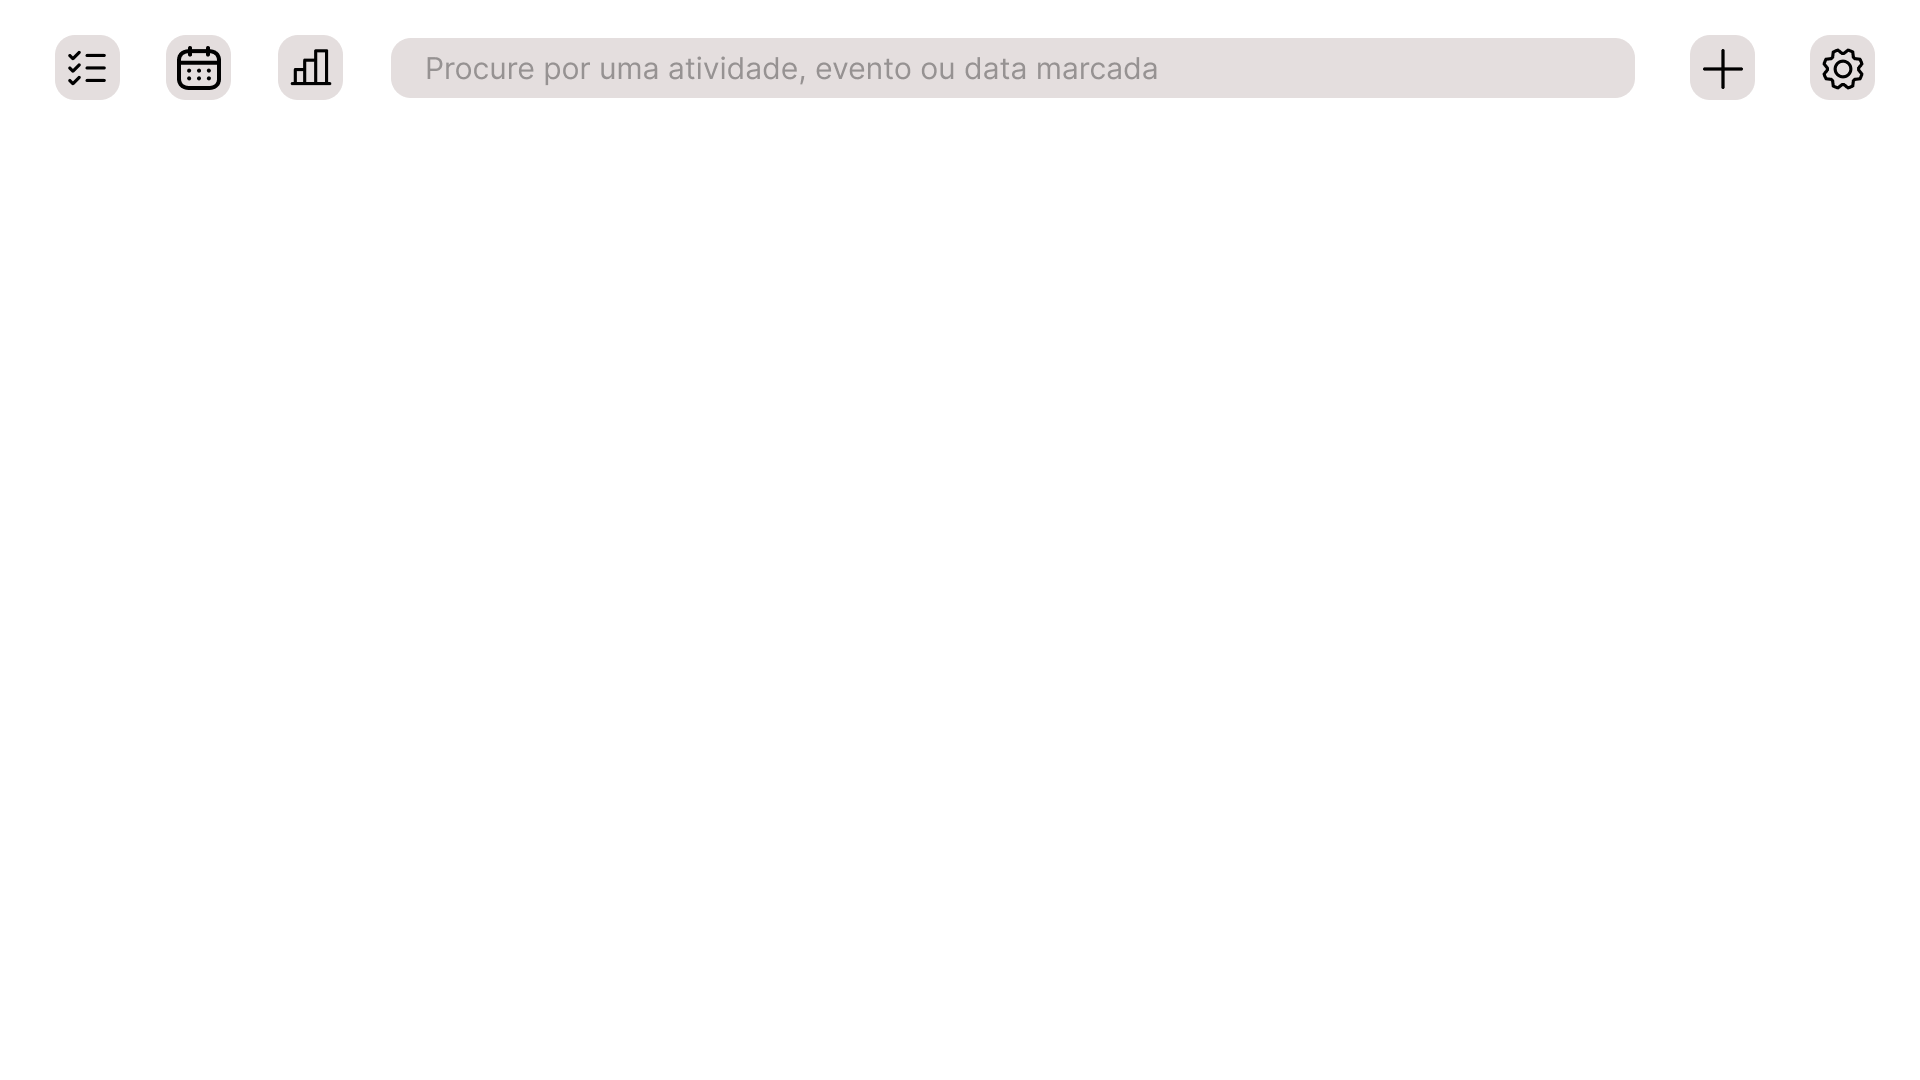
\includegraphics[scale=0.20]{prototypes/white/Main Window.png}
		\caption{JFrame principal - Modo Claro}
	\end{figure}

	\item Calendário de Tasks
	\begin{figure}[H]
		\centering
		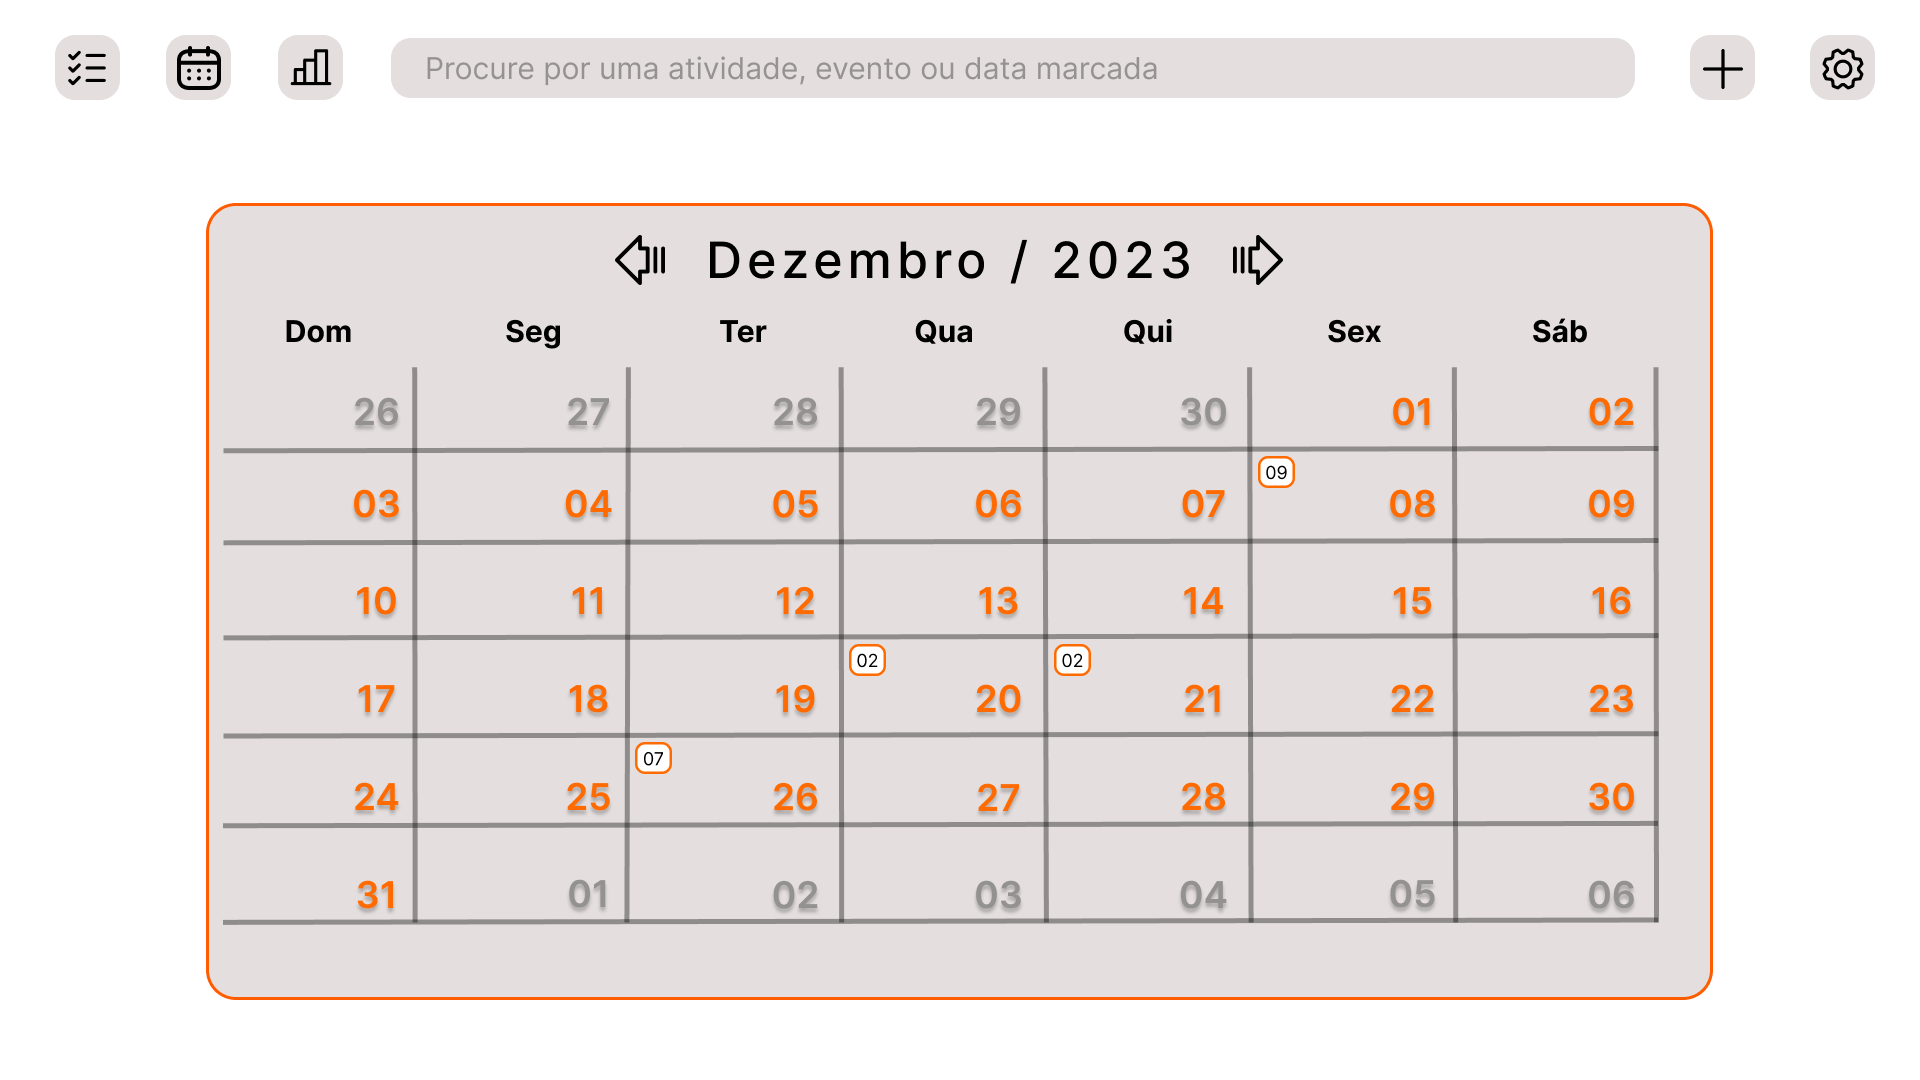
\includegraphics[scale=0.20]{prototypes/white/Calendar Panel Window.png}
		\caption{JPanel Calendário - Modo Claro}
	\end{figure}	

	\item Estatísticas Gerais
	\begin{figure}[H]
		\centering
		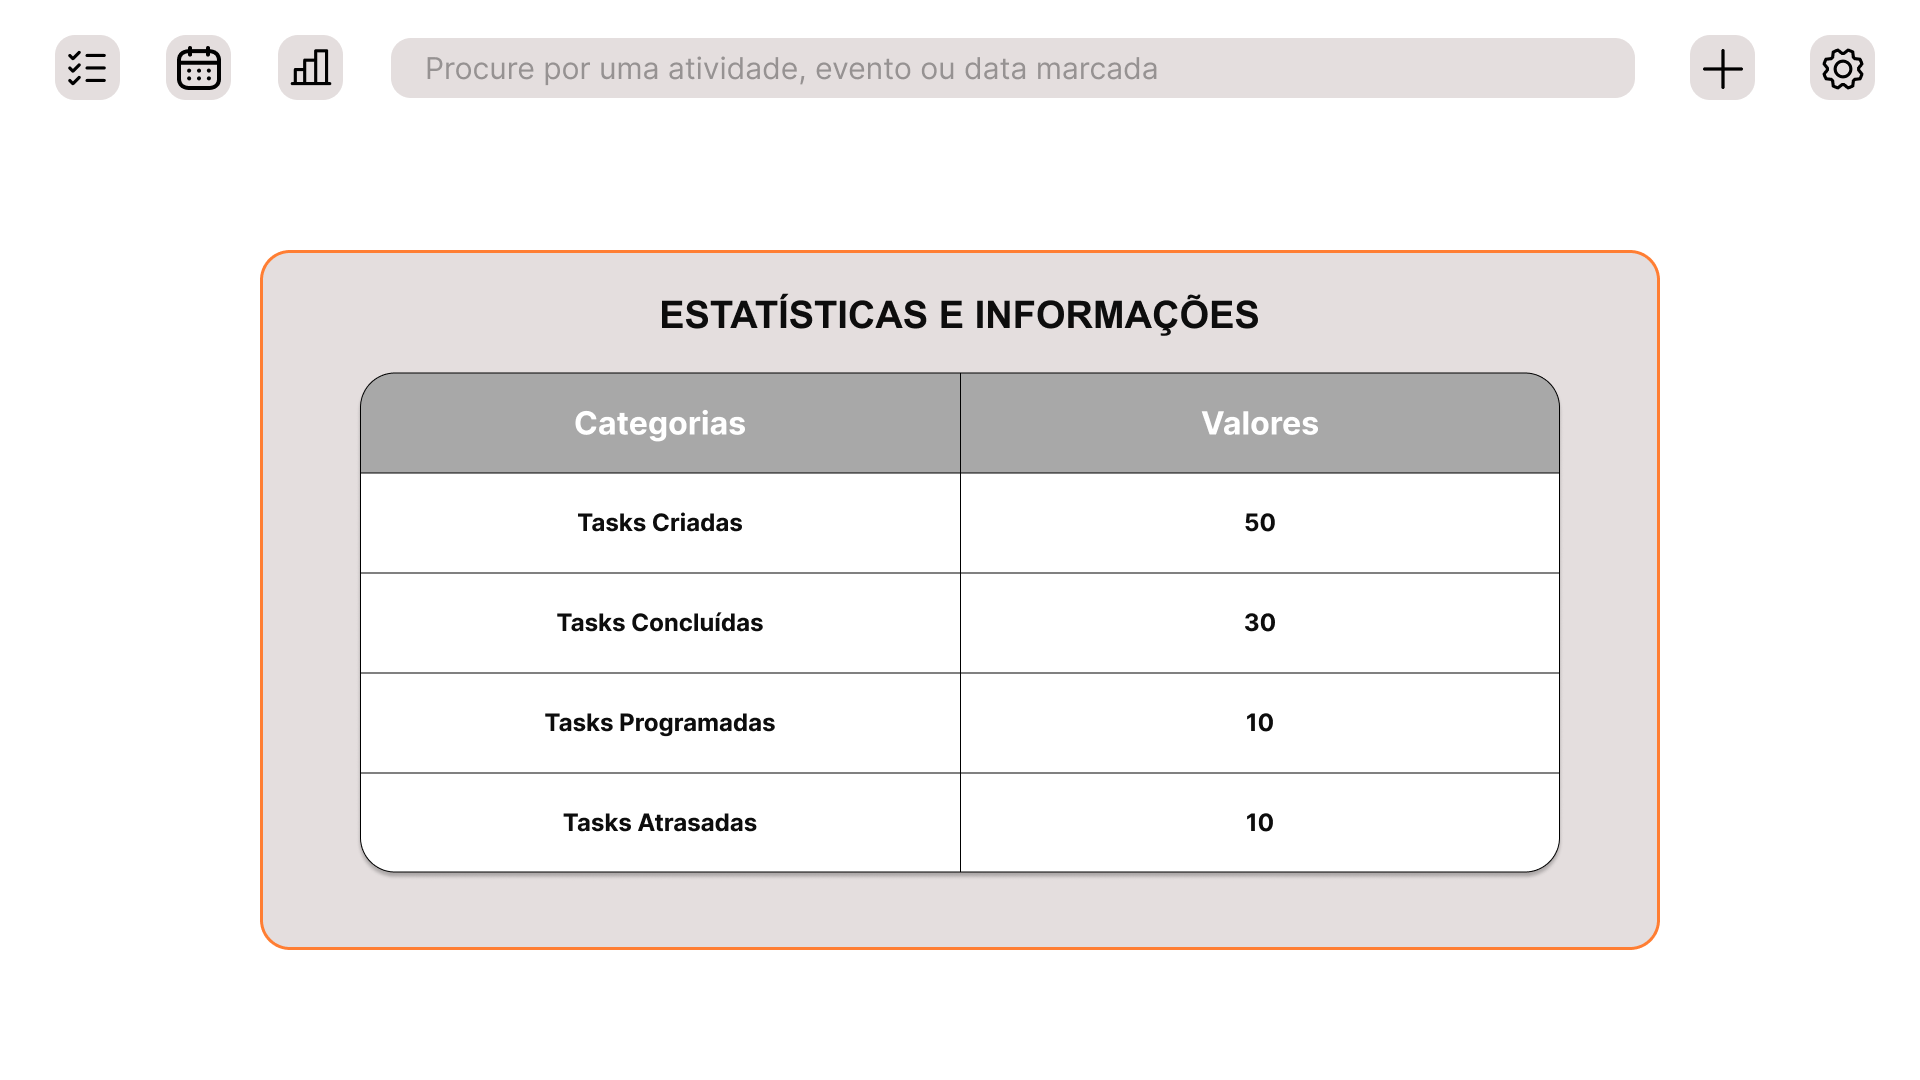
\includegraphics[scale=0.20]{prototypes/white/Stats Panel Window.png}
		\caption{JPanel de Informações e Estatísticas - Modo Claro}
	\end{figure}

	\item Tela de Configuração
	\begin{figure}[H]
		\centering
		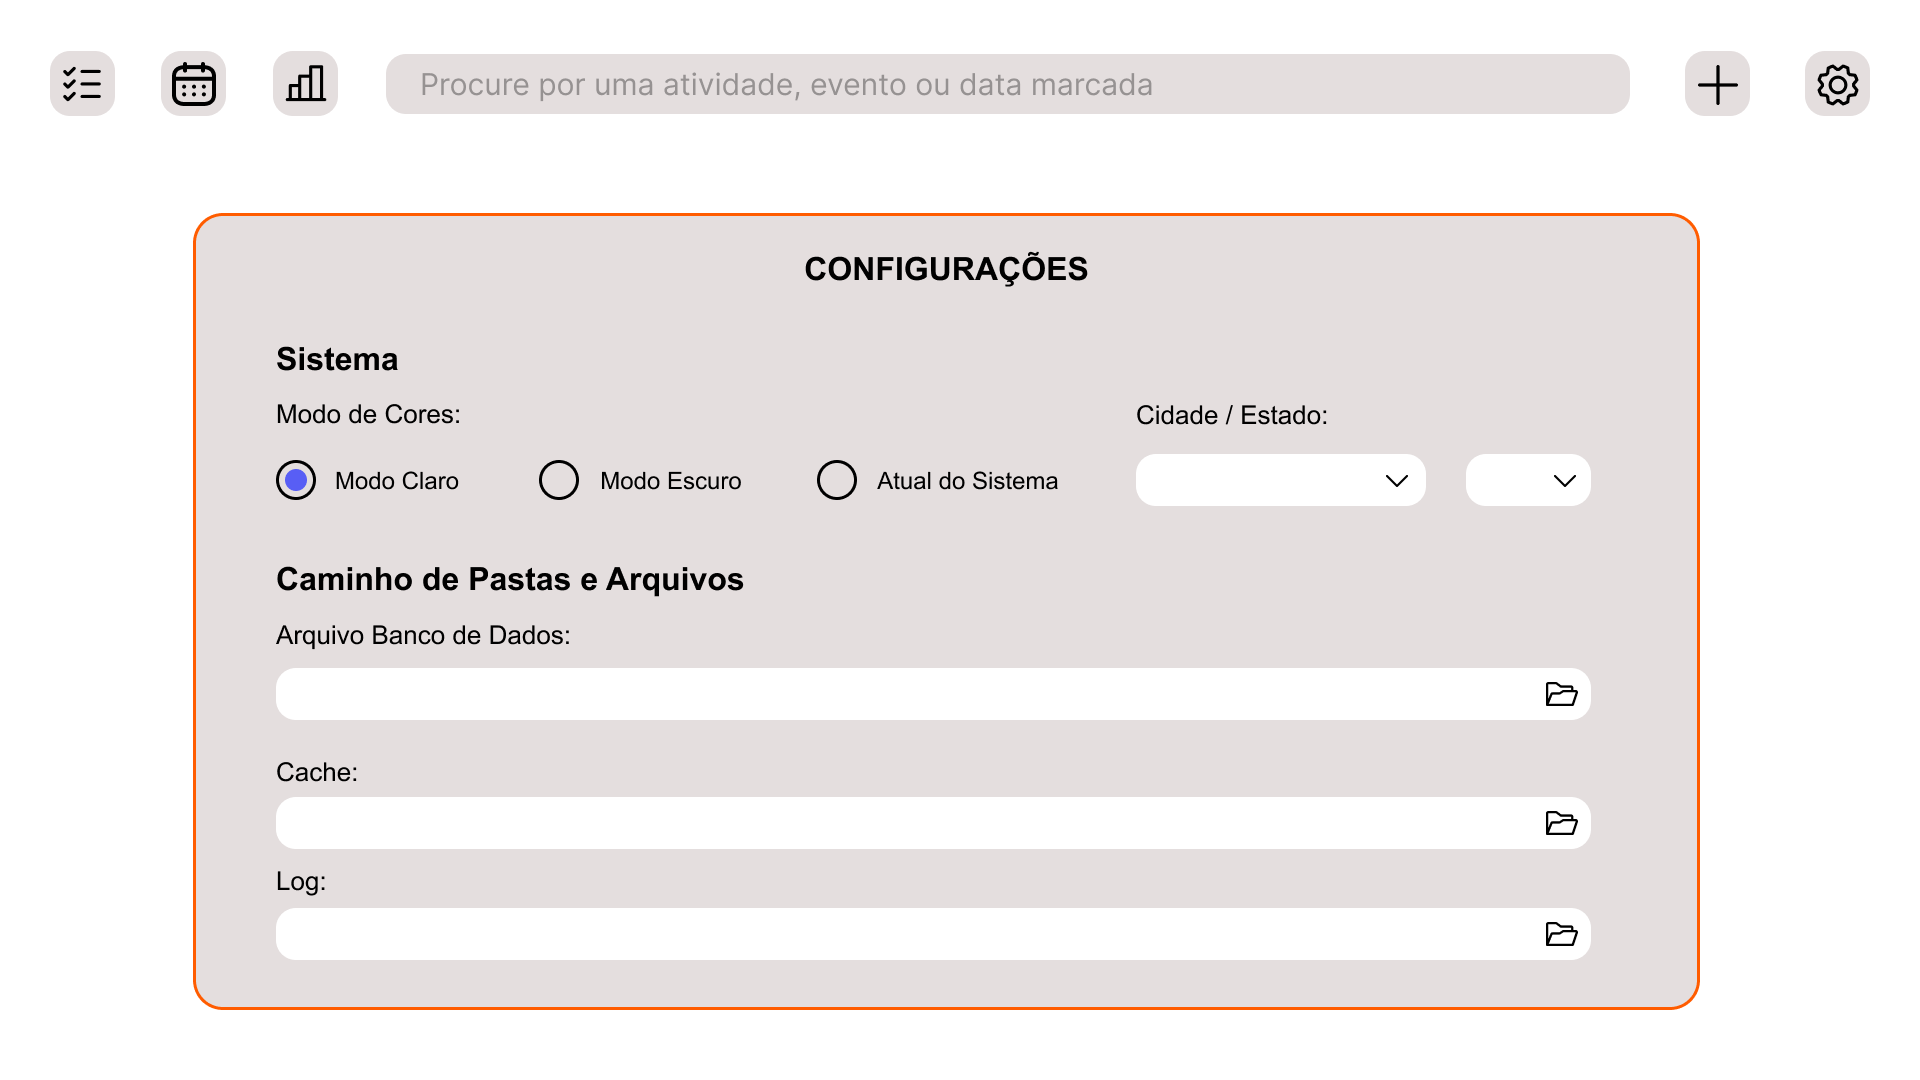
\includegraphics[scale=0.20]{prototypes/white/Config Panel Window.png}
		\caption{JPanel de Configurações - Modo Claro}
	\end{figure}

	\item Tela de Adição de Tasks
	\begin{figure}[H]
		\centering
		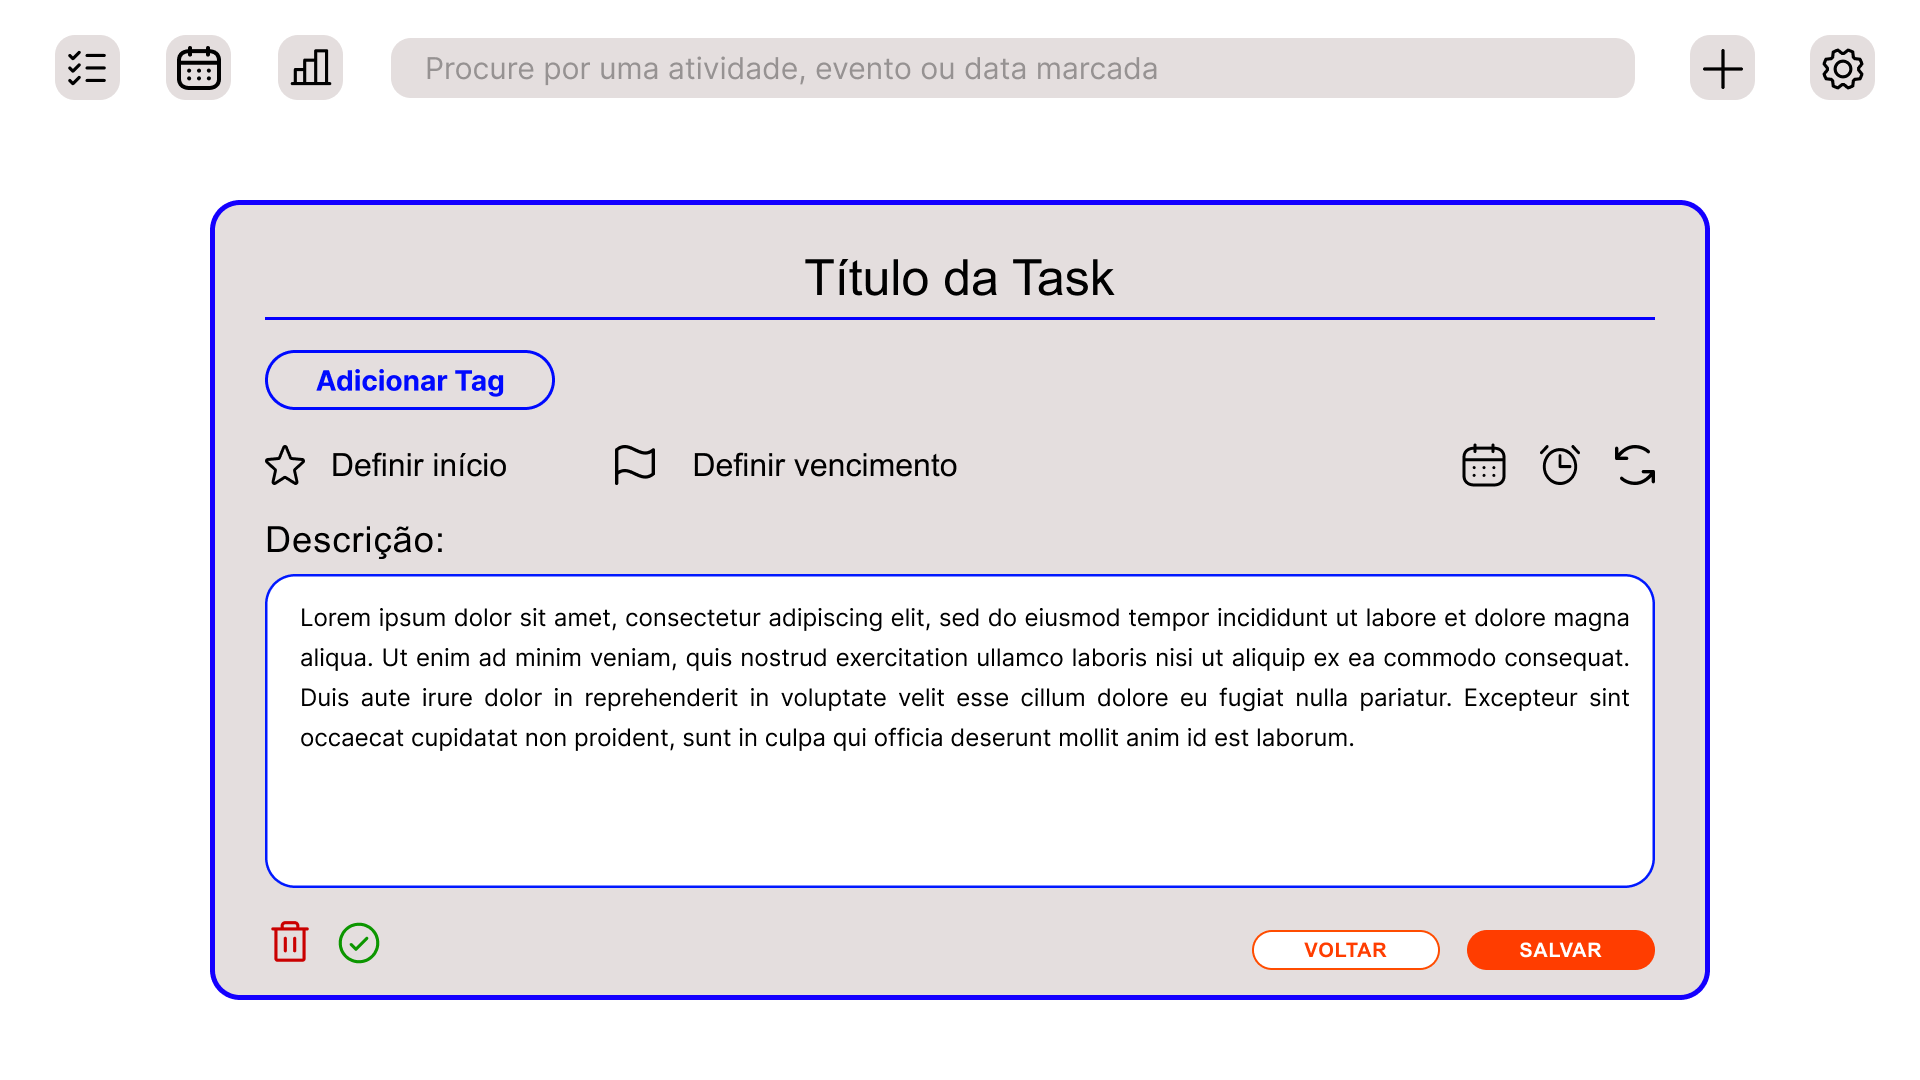
\includegraphics[scale=0.20]{prototypes/white/Add Task Panel Window.png}
		\caption{JPanel de Adição de Tasks - Modo Claro}
	\end{figure}

	\item Tela de Edição de Tasks
	\begin{figure}[H]
		\centering
		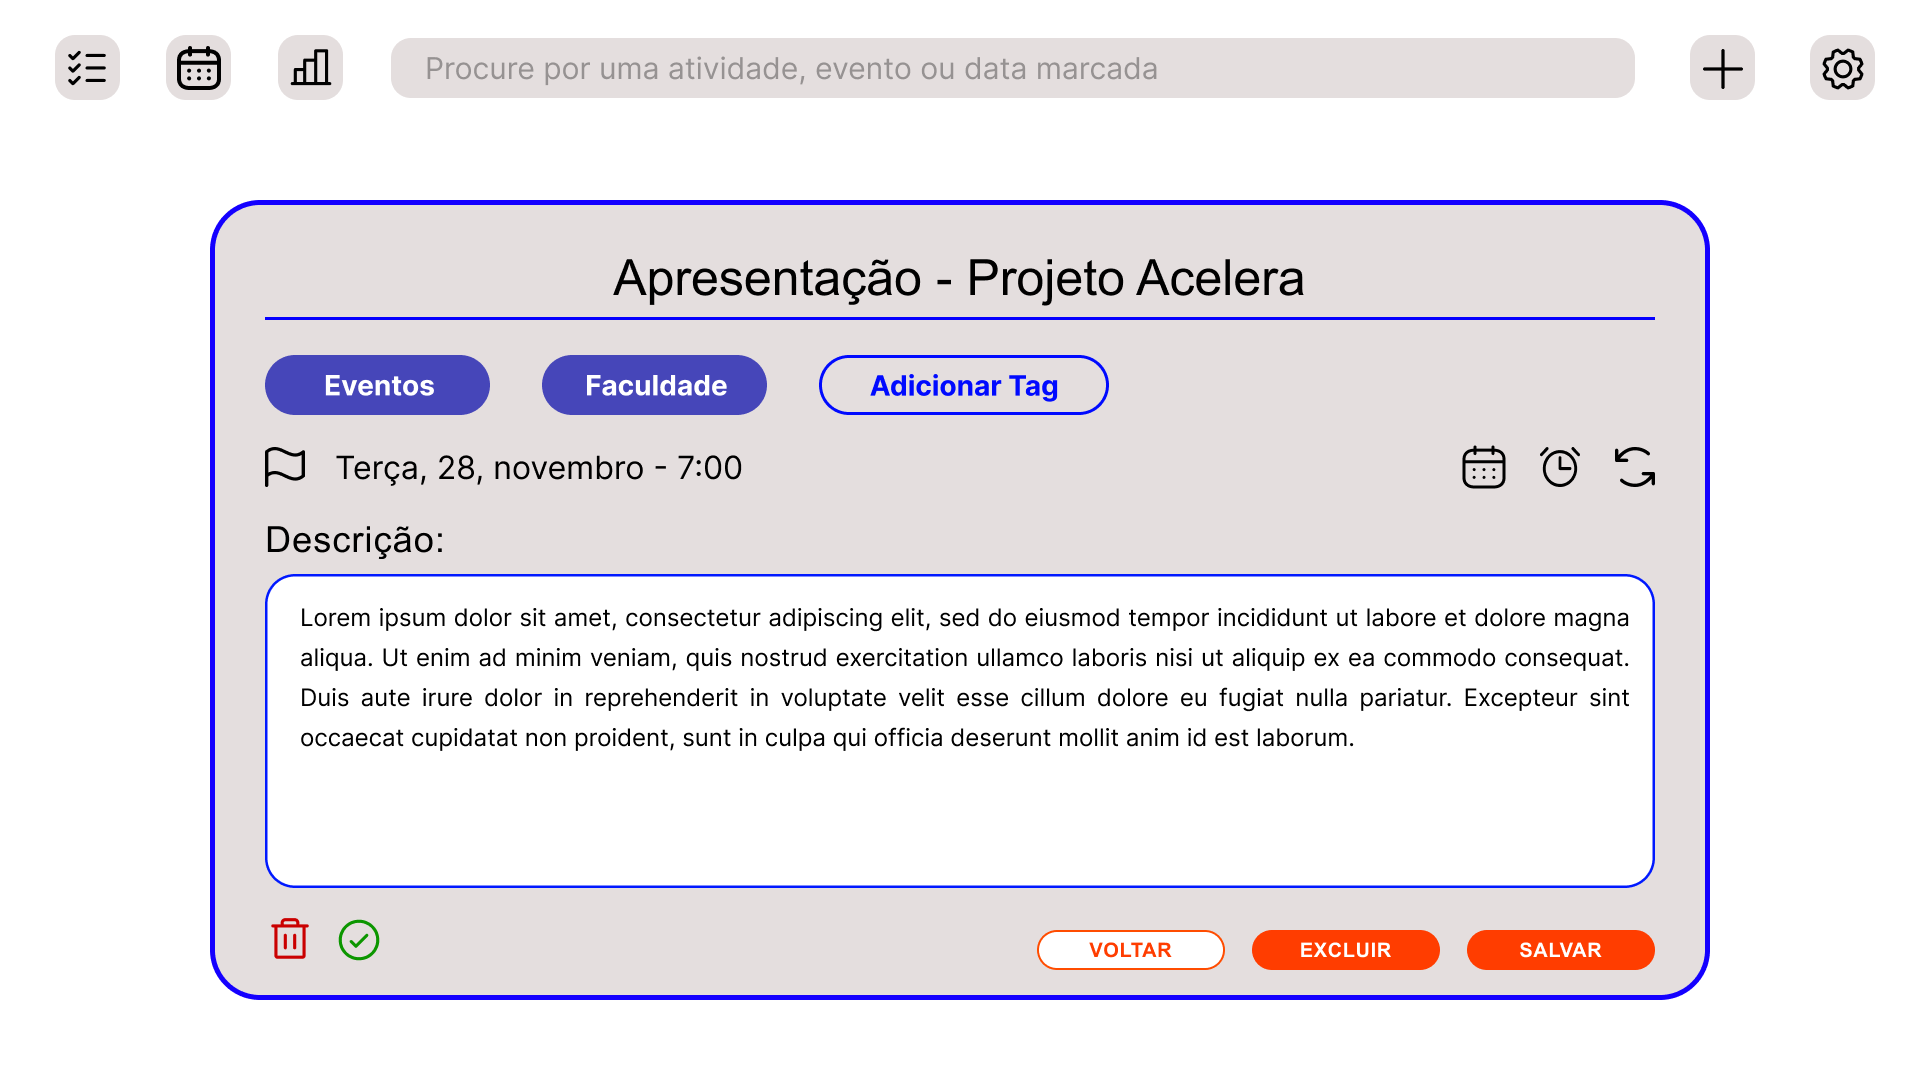
\includegraphics[scale=0.20]{prototypes/white/Edit Task Panel Window.png}
		\caption{JPanel de Edição de Tasks - Modo Claro}
	\end{figure}
\end{itemize}	

\subsubsection{Tema Escuro}
Telas com tema escuro são aquelas que apresentam cores mais escuras, como o preto, o cinza escuro, o azul escuro, entre outros. A ideia de um tema escuro é a de que o usuário possa utilizar o sistema em ambientes com iluminação mais fraca, como em ambientes internos, por exemplo.
\begin{itemize}
	\item Tema Principal
	\begin{figure}[H]
		\centering
		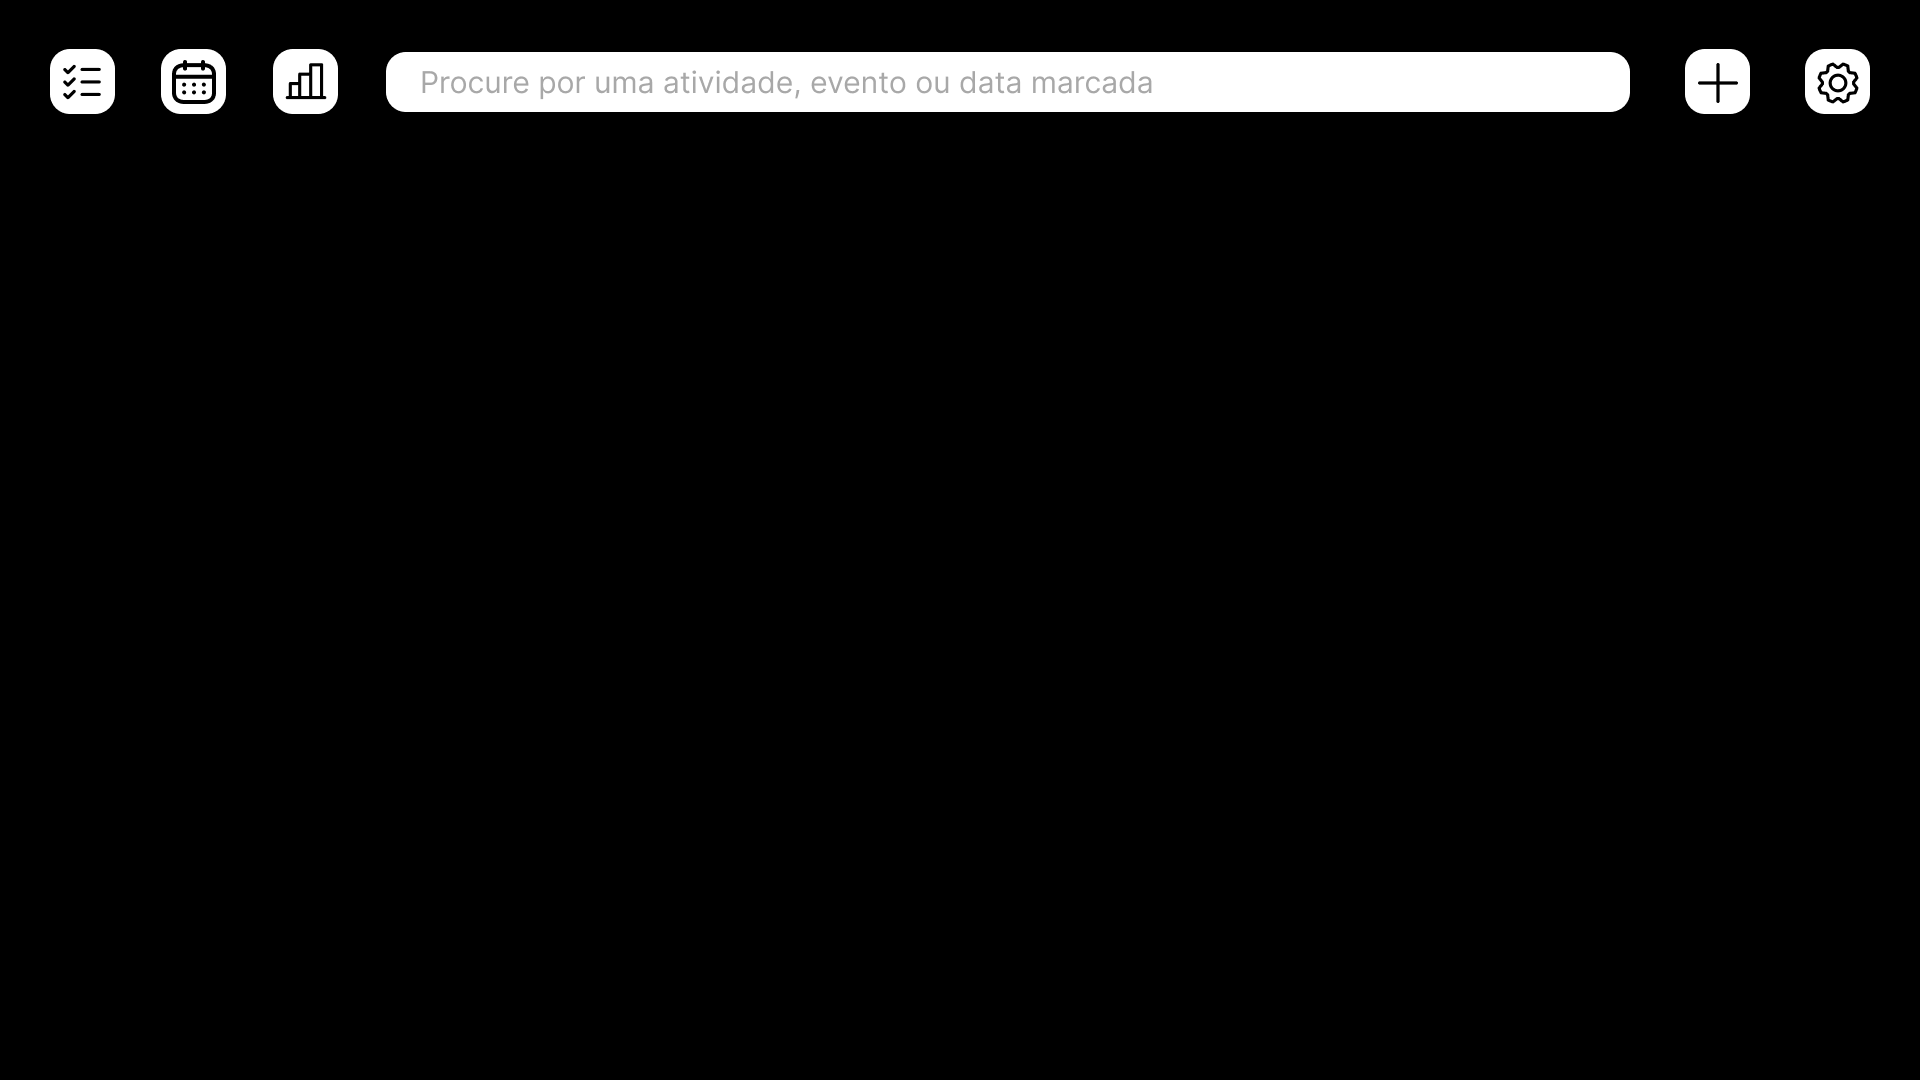
\includegraphics[scale=0.20]{prototypes/dark/Main Window.png}
		\caption{JFrame principal - Modo Escuro}
	\end{figure}

	\item Calendário de Tasks
	\begin{figure}[H]
		\centering
		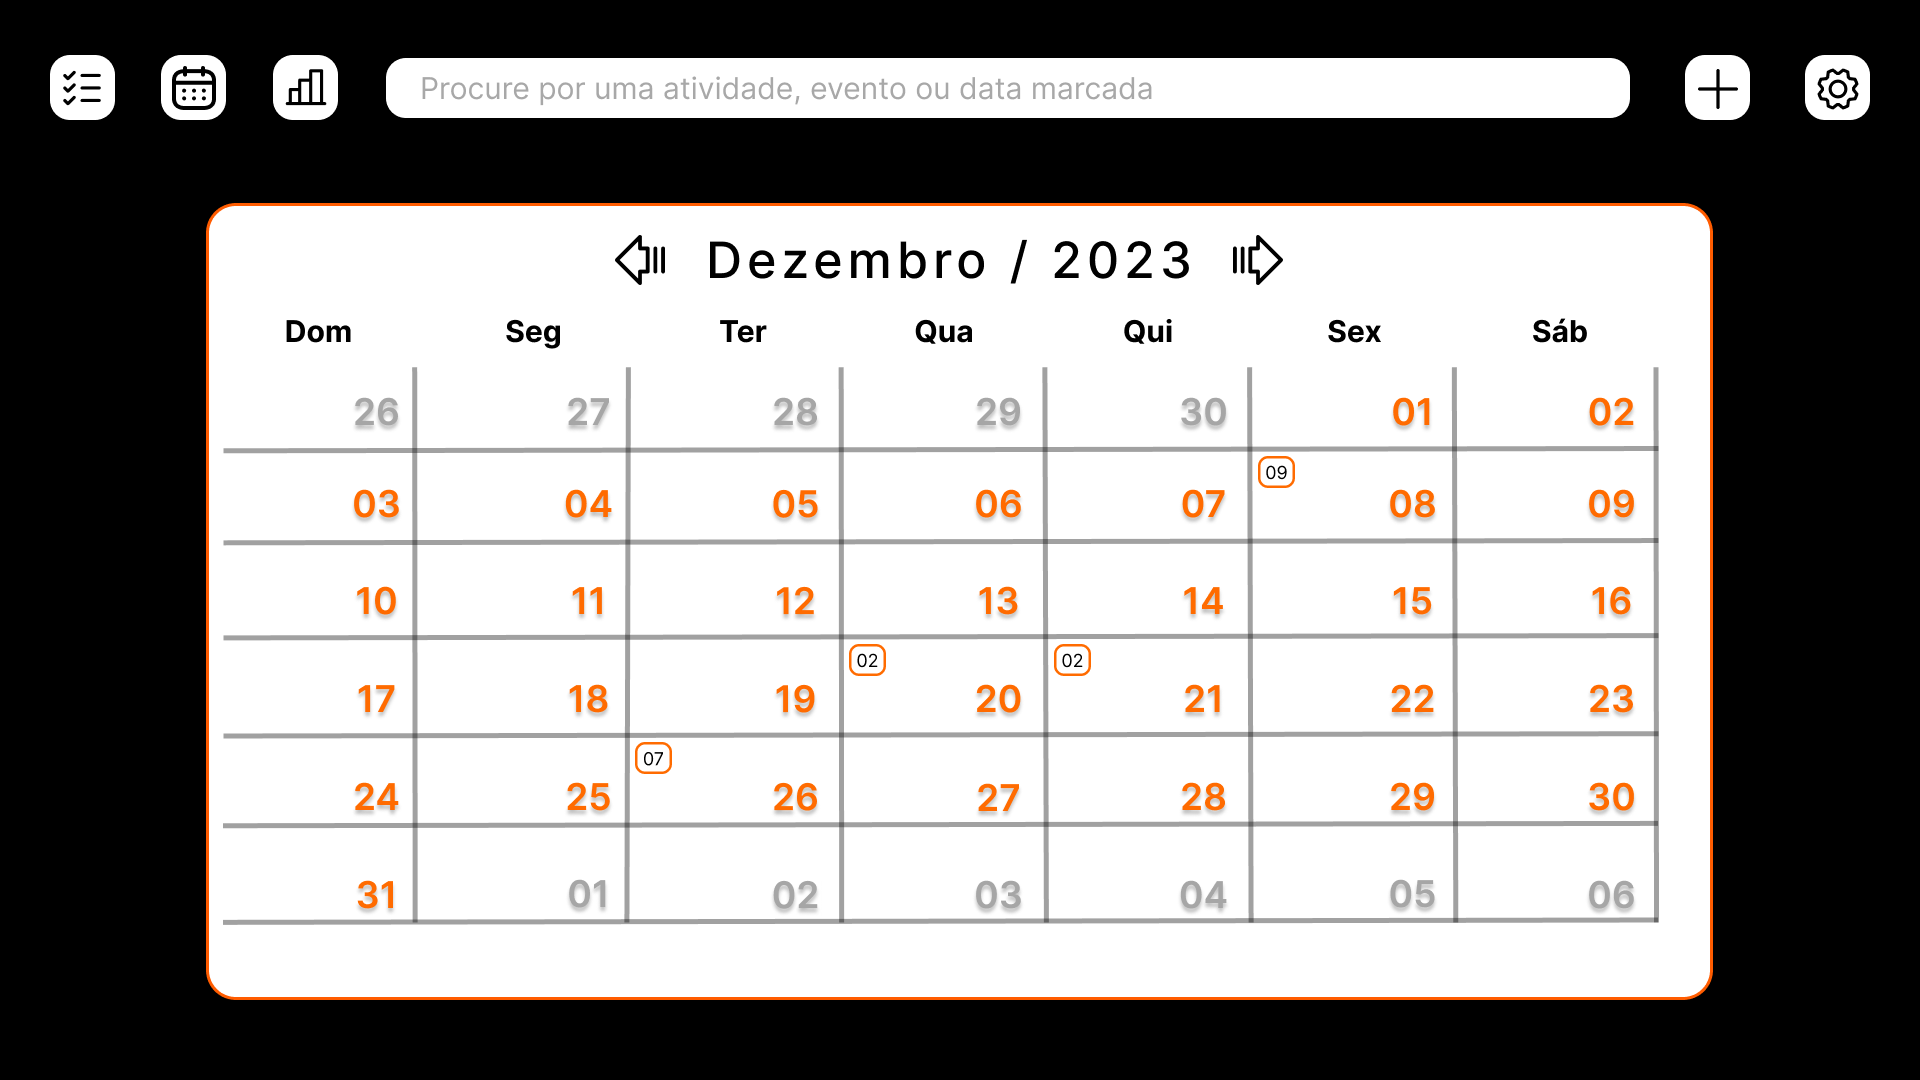
\includegraphics[scale=0.20]{prototypes/dark/Calendar Panel Window.png}
		\caption{JPanel Calendário - Modo Escuro}
	\end{figure}	

	\item Estatísticas Gerais
	\begin{figure}[H]
		\centering
		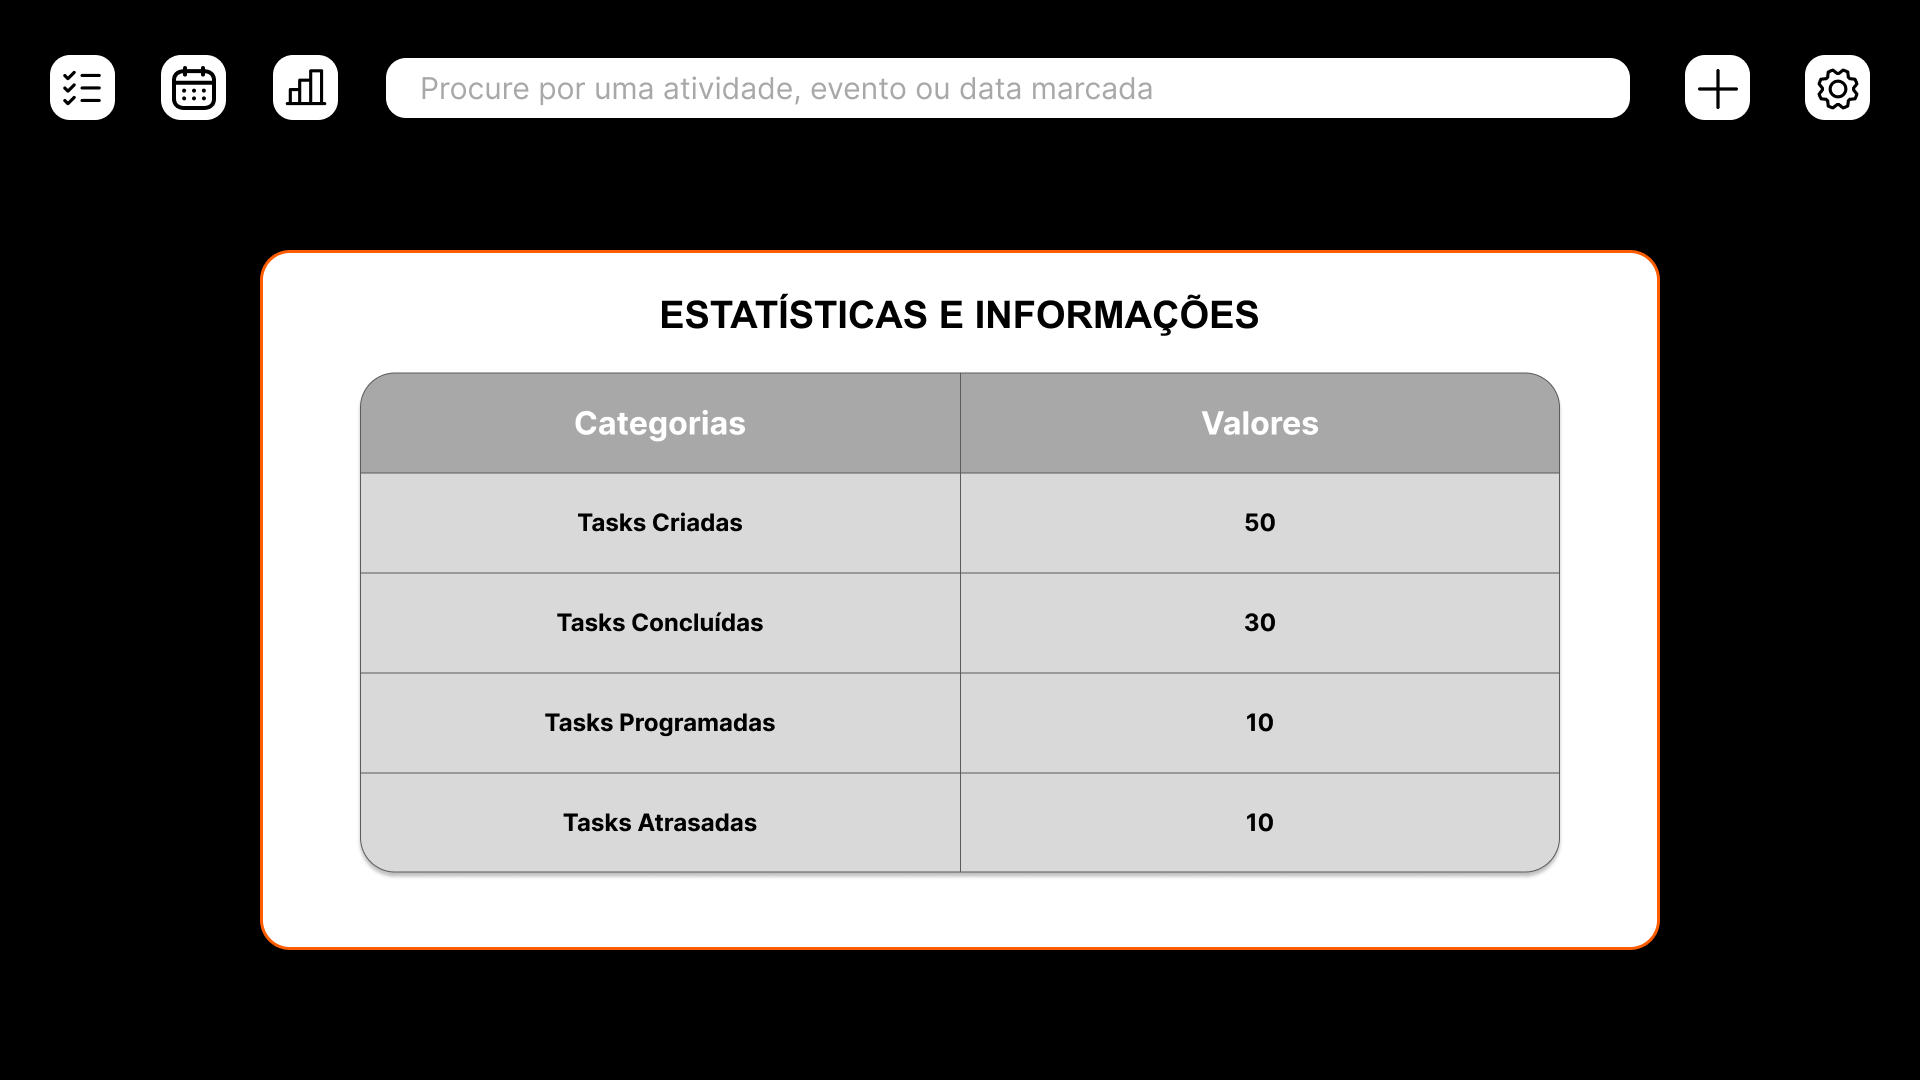
\includegraphics[scale=0.20]{prototypes/dark/Stats Panel Window.png}
		\caption{JPanel de Informações e Estatísticas - Modo Escuro}
	\end{figure}

	\item Tela de Configuração
	\begin{figure}[H]
		\centering
		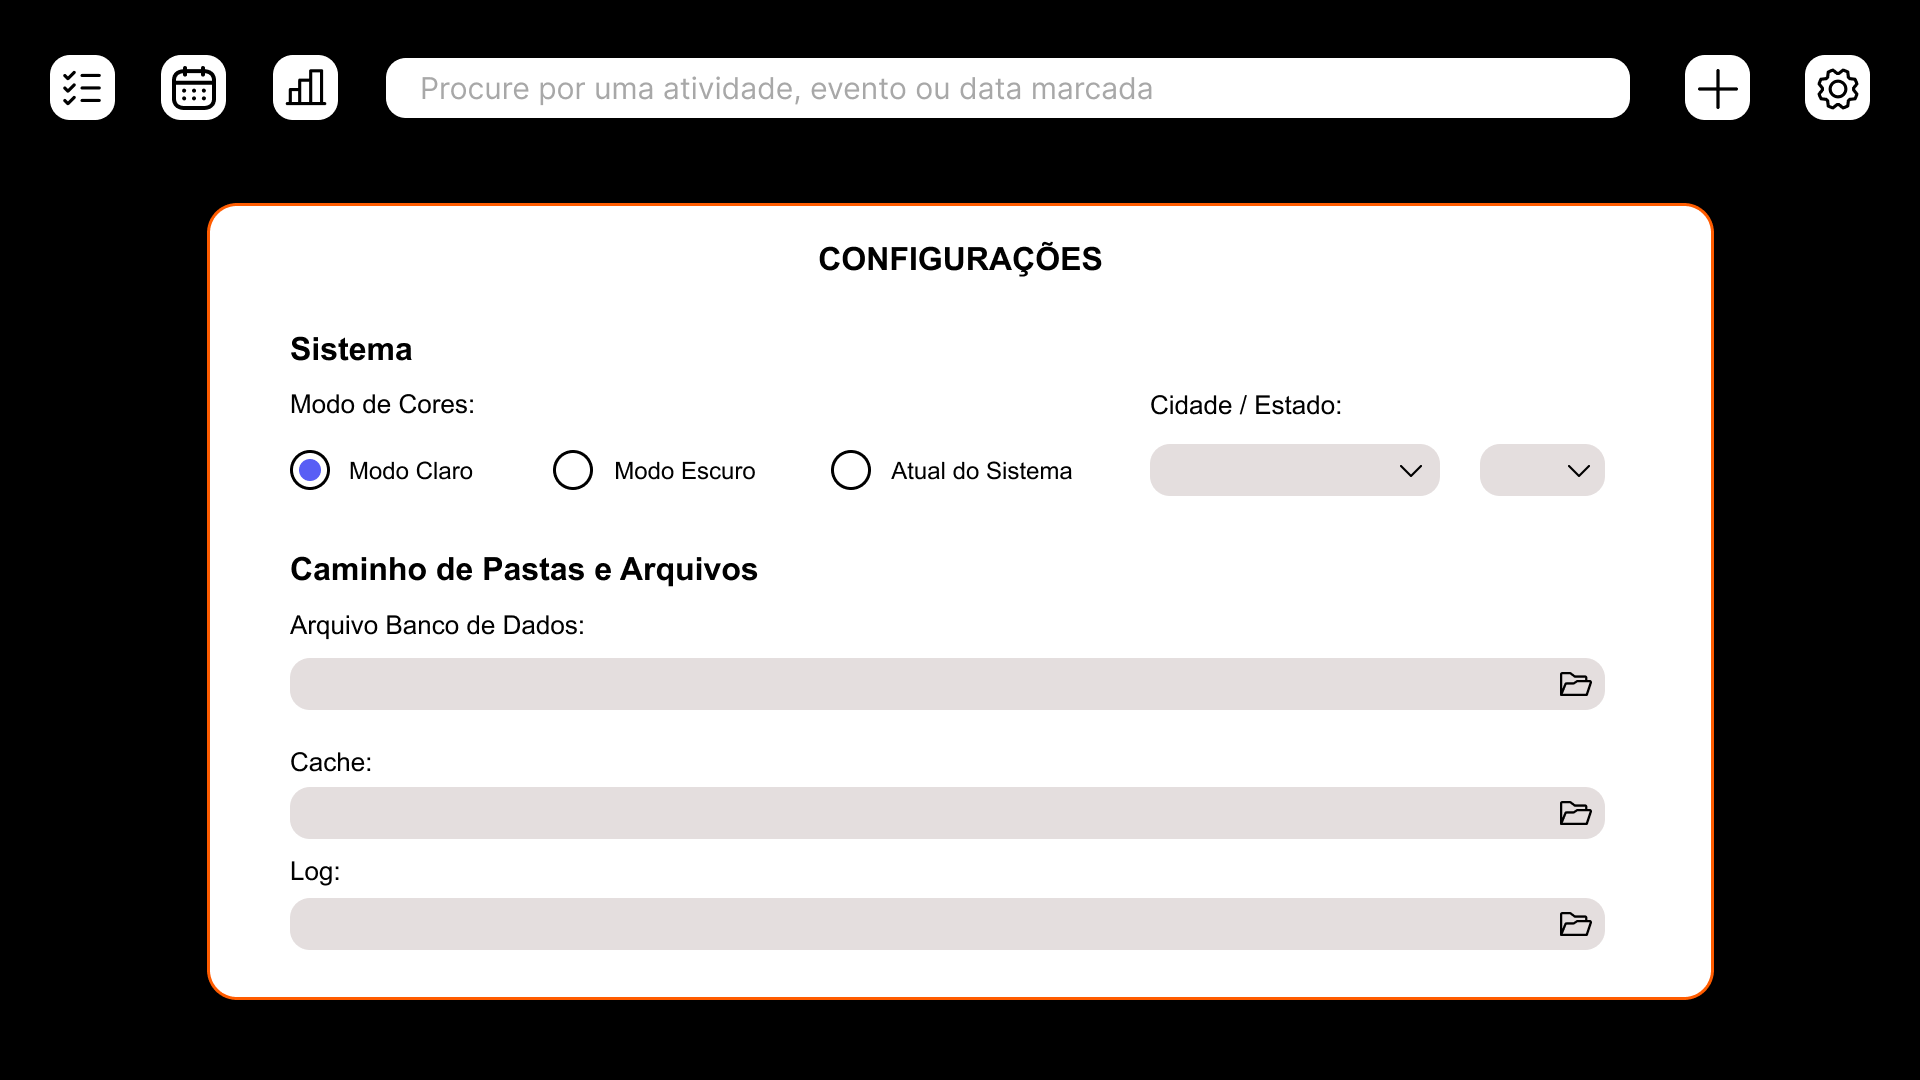
\includegraphics[scale=0.20]{prototypes/dark/Config Panel Window.png}
		\caption{JPanel de Configurações - Modo Escuro}
	\end{figure}

	\item Tela de Adição de Tasks
	\begin{figure}[H]
		\centering
		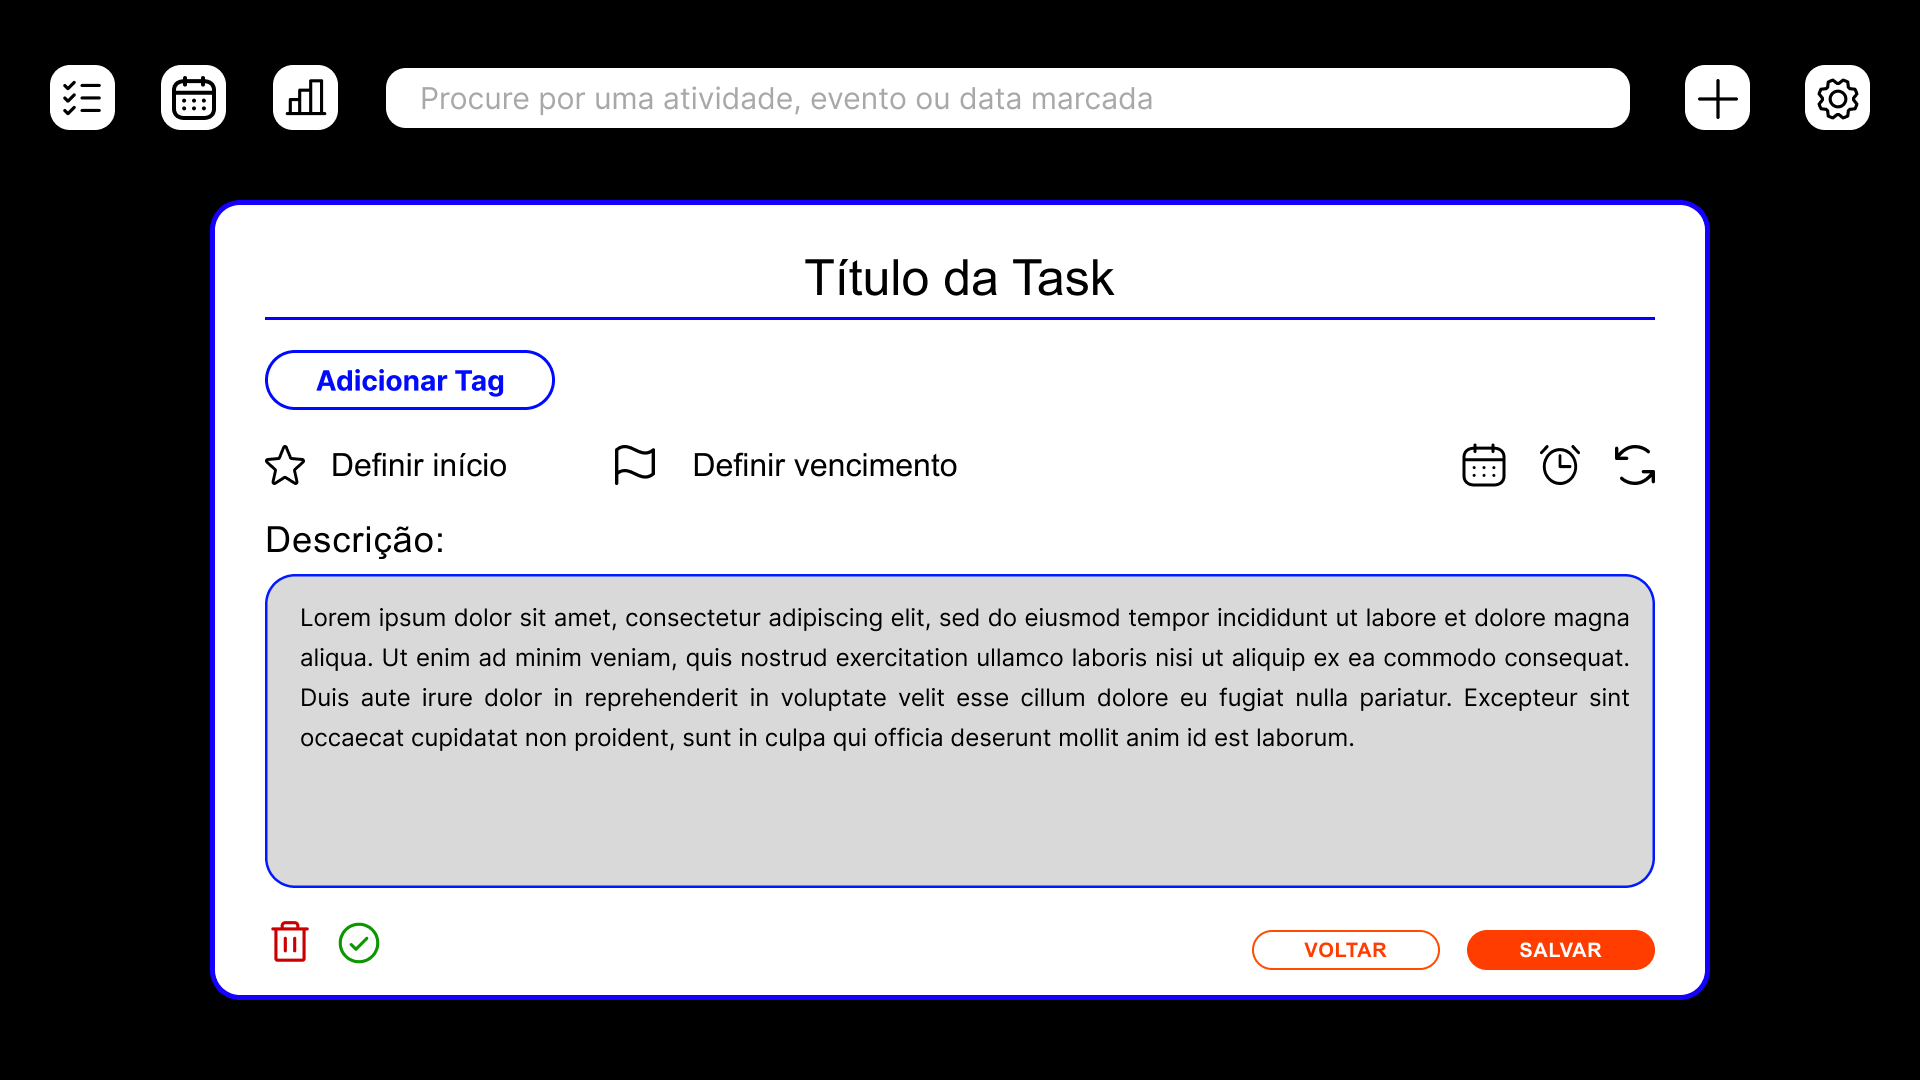
\includegraphics[scale=0.20]{prototypes/dark/Add Task Panel Window.png}
		\caption{JPanel de Adição de Tasks - Modo Escuro}
	\end{figure}

	\item Tela de Edição de Tasks
	\begin{figure}[H]
		\centering
		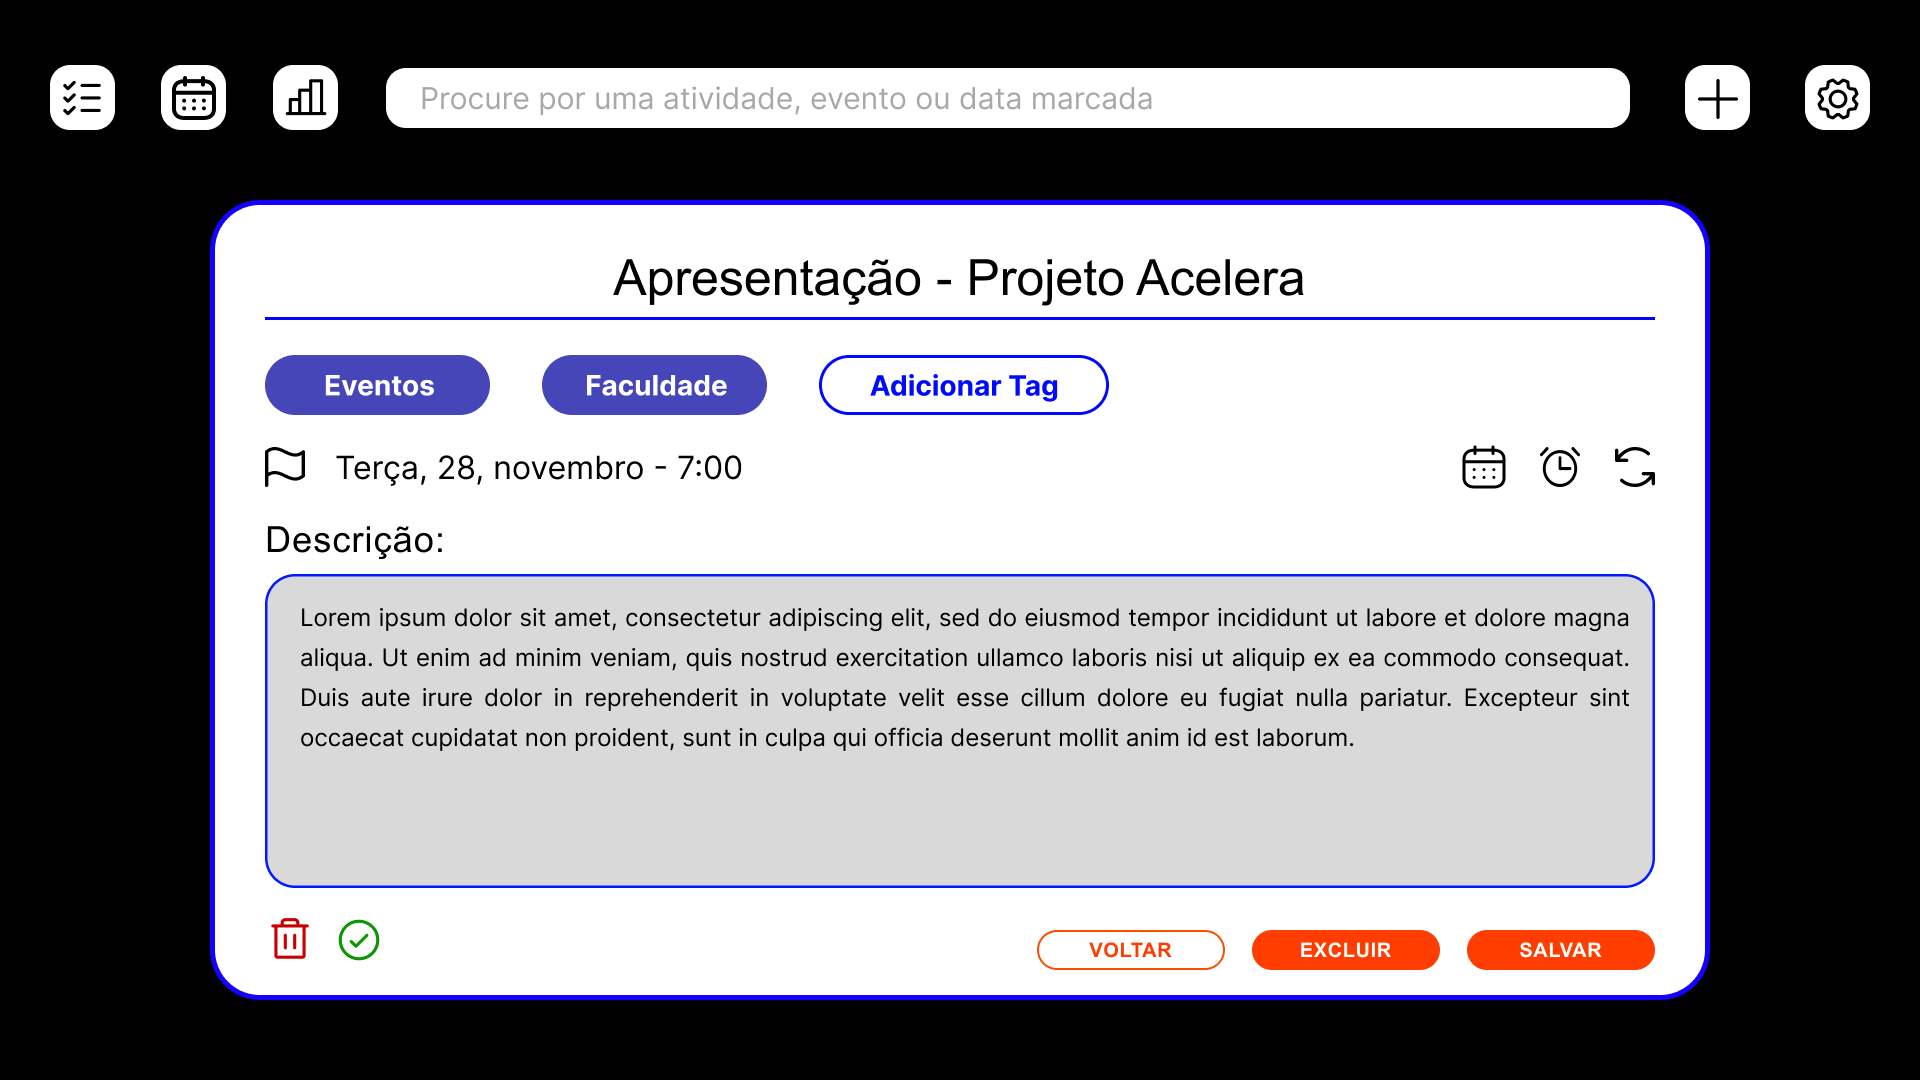
\includegraphics[scale=0.20]{prototypes/dark/Edit Task Panel Window.png}
		\caption{JPanel de Edição de Tasks - Modo Escuro}
	\end{figure}
\end{itemize}

A seguir, temos outros JFrames que servirão como modais, ou pequenas telas informativas e de confirmação de ações, que serão apresentadas sobre a tela principal, e que serão apresentadas em ambos os temas, claro e escuro.
\begin{itemize}
	\item Tela de Confirmação de Exclusão de Tasks
	\begin{figure}[H]
		\centering
		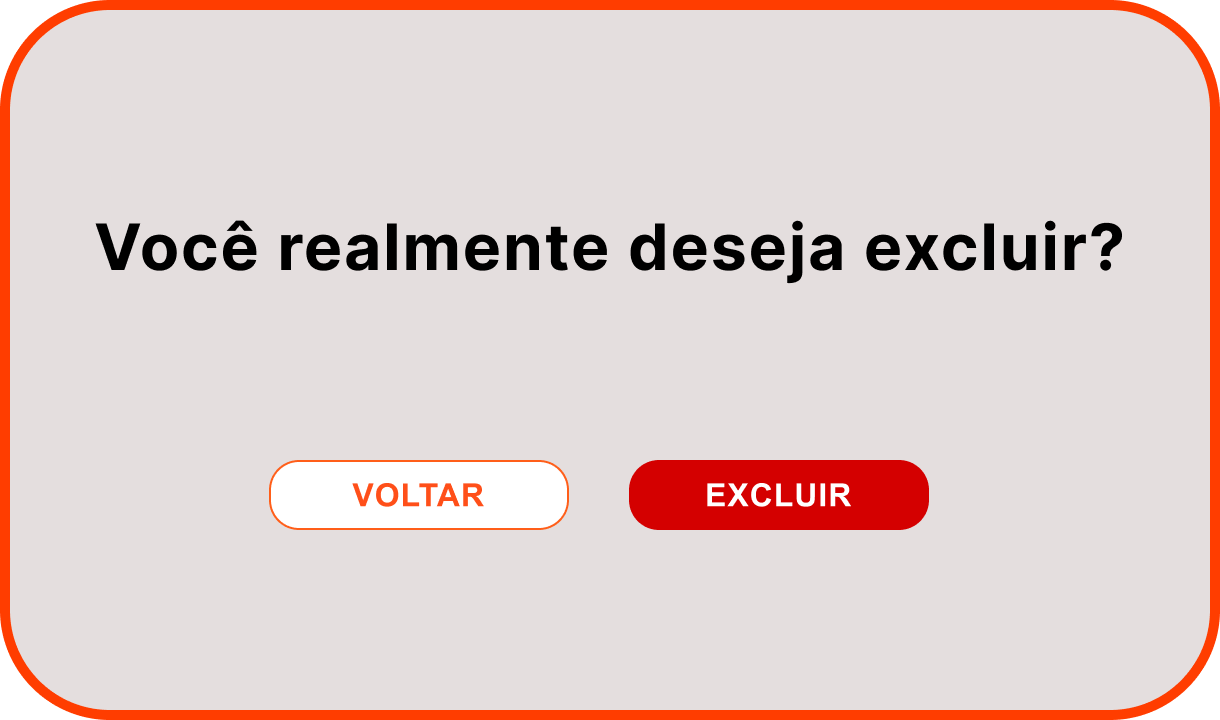
\includegraphics[scale=0.20]{prototypes/white/Modal Confirmation.png}
		\caption{JFrame de Confirmação de Exclusão de Tasks}
	\end{figure}

	\item Tela de Criação de Tags
	\begin{figure}[H]
		\centering
		\includegraphics[scale=0.20]{prototypes/white/Add Tag.png}
		\caption{JFrame de Criação de Tags}
	\end{figure}

	\item Tela de Sobre (Equipe e Sistema)
	\begin{figure}[H]
		\centering
		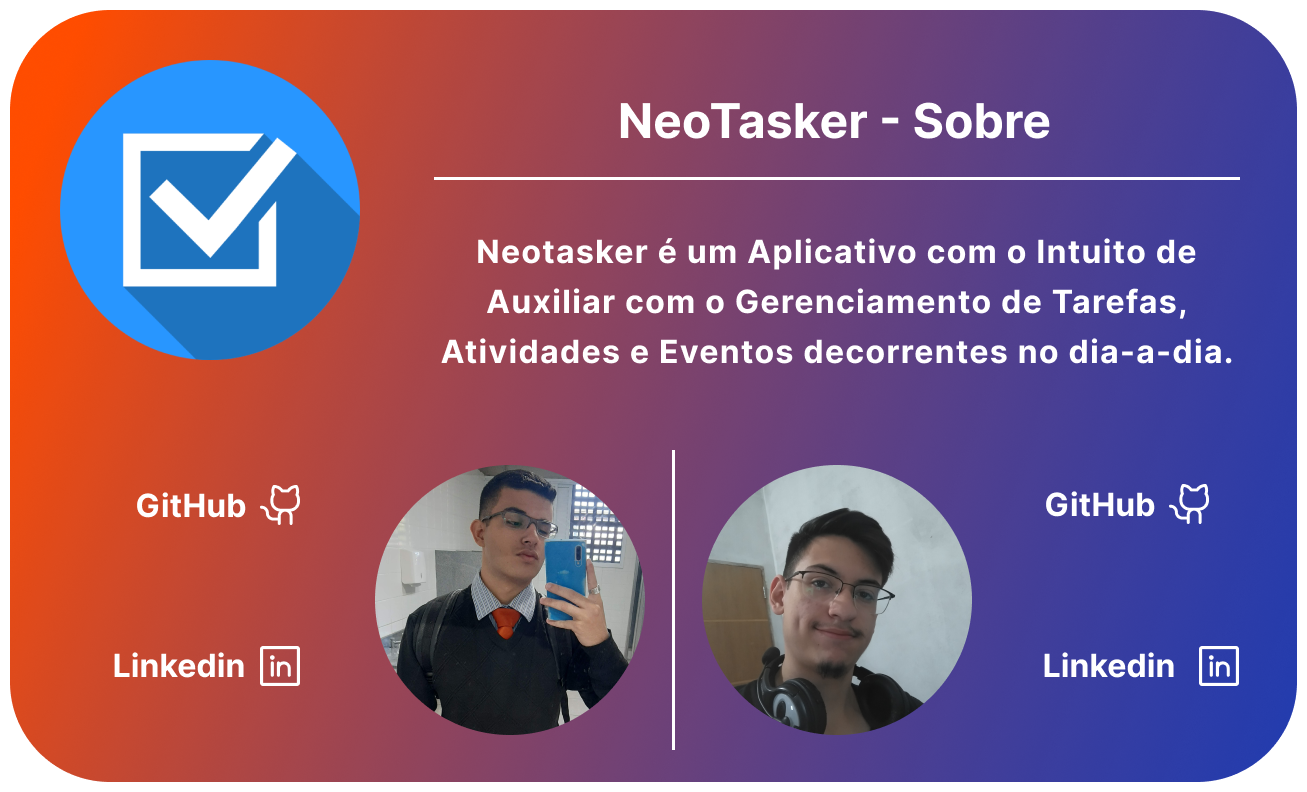
\includegraphics[scale=0.20]{prototypes/white/About Us Panel Window.png}
		\caption{JFrame de Sobre (Equipe e Sistema)}
	\end{figure}
\end{itemize}

% --- Segment: Color Palette ---
\section{Paleta de Cores do Sistema}
A paleta de cores do sistema é o conjunto de cores que serão utilizadas no sistema, tanto para o tema claro quanto para o tema escuro. É importante destacar que as cores do sistema foram escolhidas usando como base seu possíveis significados e o que elas poderiam significar para o usuário final, em diferentes situações e processos dentro do sistema.

\subsection{Sistema de Cores}

% --- Document: End ---
\end{document}
